%%%%% Güncelleme Geçmişi
%%%%% v3.5 -> 10.09.2024 (AEL)
%%%%% v3.4 -> 06.06.2020 (AEL)
%%%%% v3.3 -> 03.06.2020 (HOI)
%%%%% v3.2 -> 29.05.2019 (HOI)
%%%%% v3.1 -> 22.05.2019 (IOS)
%%%%% v3.0 -> 06.11.2018 (IOS)
%%%%% v2.0 -> 01.03.2017 (IOS)
%%%%% v1.2 -> 20.12.2016 (IOS)
%%%%% v1.1 -> 10.11.2016 (IOS)

\documentclass[a4paper,12pt,oneside,openany]{book}

%%%%%%%%%%%%%%%%%%%%%%%%%%%%%%%%%%%%%%%%%%%%%%%%%%%%%
%%%%%%%%%%%      PROJECT PARAMETERS      %%%%%%%%%%%%
%%%%%%%%%%%%%%%%%%%%%%%%%%%%%%%%%%%%%%%%%%%%%%%%%%%%%

% Project Option: "computer" or "senior"
% Report Option: "report" or "final"

% Example:   \usepackage[computer, report]{ytucestyle}
%            \usepackage[senior, final]{ytucestyle}

\usepackage[computer, final]{ytucestyle}

\usepackage{listings}
\usepackage{float}
\lstset{
  basicstyle=\ttfamily\small,
  frame=lines,
  breaklines=true,
  postbreak=\mbox{\textcolor{red}{$\hookrightarrow$}\space},
  literate={ğ}{{\u{g}}}1 {ü}{{\"u}}1 {ş}{{\c{s}}}1 {ı}{{\i}}1 {ö}{{\"o}}1 {ç}{{\c{c}}}1 {Ğ}{{\u{G}}}1 {Ü}{{\"U}}1 {Ş}{{\c{S}}}1 {İ}{{\.I}}1 {Ö}{{\"O}}1 {Ç}{{\c{C}}}1
}
\usepackage{tikz}
\usetikzlibrary{positioning,arrows.meta}
\usepackage{pgfplots}
\pgfplotsset{compat=1.18}
\usepackage{pgfgantt} % <-- Gantt şeması için eklendi
\usepackage{multirow}
%%%%%%%%%%%%%%%%%%%%%%%%%%%%%%%%%%%%%%%%%%%%%%%%%%%%%
%%%%%%%%%%%         REFERENCES       %%%%%%%%%%%%%%%%
%%%%%%%%%%%%%%%%%%%%%%%%%%%%%%%%%%%%%%%%%%%%%%%%%%%%%
\addbibresource{references.bib} 

\begin{document}
%%%%%%%%%%%%%%%%%%%%%%%%%%%%%%%%%%%%%%%%%%%%%%%%%%%%%
%%%%%%%%%%%         FRONT PAGES      %%%%%%%%%%%%%%%%
%%%%%%%%%%%%%%%%%%%%%%%%%%%%%%%%%%%%%%%%%%%%%%%%%%%%%
% Aşağıdaki değeri {1} AR-GE 1, YAZILIM 2 veya LATEX TUTORİAL 3 olarak değiştirin 
\newcommand{\projecttype}{2}
\ifnum\projecttype=3
\input {LatexTutorial/Warning.tex}
\else
\input {frontPages.tex}
\fi
%%%%%%%%%%%%%%%%%%%%%%%%%%%%%%%%%%%%%%%%%%%%%%%%%%%%%
%%%%%%%%%%%%%%%      CHAPTERS     %%%%%%%%%%%%%%%%%%%
%%%%%%%%%%%%%%%%%%%%%%%%%%%%%%%%%%%%%%%%%%%%%%%%%%%%%
\ifnum\projecttype=1
\chapter{GİRİŞ}
\label{ch:giris}

% --- 1.1 ---

\label{sec:ajan-mimari}

Modern yapay zeka uygulamalarının temelinde, devasa metin ve kod veri kümeleri üzerinde eğitilmiş Büyük Dil Modelleri (LLM) yer almaktadır. Bu modeller, kendilerine sunulan bilgiyi anlama ve üretme konusunda yüksek kapasiteye sahip olsalar da, tek başlarına karmaşık ve çok aşamalı görevleri yerine getirmede sınırlı kalmaktadır. Bu noktada ajan tabanlı sistemler devreye girmektedir. Bir ajan, LLM'yi karar alma çekirdeği olarak kullanır; hedefe yönelik planlama yapar, dosya okuma veya kod yürütme gibi yardımcı araçları etkinleştirir ve çevreden aldığı geri bildirime göre stratejisini günceller.

Örneğin finans teknolojileri alanında çalışan bir yazılım mühendisinin, on binlerce dosyadan oluşan yeni bir ödeme altyapısına katıldığını düşünelim. Geliştiricinin mimariyi anlaması, iş akışlarını kavraması ve basit bir değişikliği güvenle uygulayabilmesi çoğu zaman haftalar almaktadır. İnsan gözetiminde yürüyen bu uzun uyum sağlama süreci, kod tabanından yapılandırılmış bilgi çıkarabilen otonom sistemlerin yokluğunda daha da uzamakta; iş devri ve bakım maliyetleri yükselmektedir.

Bu mimarilerin en belirgin teknik kısıtlaması, LLM'lerin "bağlam penceresi" olarak bilinen veri işleme sınırıdır. Bir model aynı anda yalnızca sınırlı miktarda bilgiyi hafızasında tutabilir. Dolayısıyla kapsamlı bir yazılım projesinin tamamını tek seferde değerlendirmek geleneksel ajan yaklaşımlarıyla mümkün olamamaktadır.


Ajan tabanlı sistemler, yazılım geliştirme yaşam döngüsünün (SDLC) birçok aşamasını otomatize etme potansiyeline sahiptir. Bu sistemler, basit kod tamamlama araçlarının çok ötesine geçerek aktif roller üstlenmeye başlamıştır. Güncel uygulama alanları arasında şunlar bulunmaktadır:

\begin{itemize}
    \item \textbf{Otomatik Hata Ayıklama (Debugging):} Bir kod tabanındaki hataları tespit etmek için test senaryoları yürütebilen, günlük (log) dosyalarını analiz edebilen ve hatanın kaynağını belirleyebilen ajanlar.
    \item \textbf{Talep Üzerine Kod Üretimi:} "Kullanıcılar için bir giriş (login) sayfası oluştur" gibi doğal dil taleplerini alıp, gerekli dosya yapılarını ve kod bloklarını üreten sistemler.
    \item \textbf{Mevcut Kodun Yeniden Yapılandırılması (Refactoring):} Verimsiz veya eski kod standartlarına göre yazılmış bölümleri analiz edip, daha performanslı veya modern eşdeğerleriyle güncelleyen ajanlar.
    \item \textbf{Kod Analizi ve Dokümantasyon:} Bu projenin de odak noktası olan, mevcut bir kod tabanını inceleyerek sistemin mimarisini, veri akışlarını ve bileşenlerin sorumluluklarını anlatan teknik dokümantasyon üreten sistemler.
\end{itemize}


Yazılım geliştirme süreçlerinde, geniş ve yabancı bir kod tabanını anlamak, yazılım geliştiricilerin karşılaştığı en önemli zorluklardan biridir. Yeni bir geliştiricinin bir projeye dahil olması  veya tecrübeli bir geliştiricinin projenin daha önce dokunmadığı bir bölümüne müdahale etmesi gerektiğinde, mevcut dokümantasyon genellikle eksik, güncel olmayan veya yüzeysel kalmaktadır. Bu durum, projelere adaptasyon sürecinin haftalar, hatta aylar sürmesine neden olarak ciddi bir zaman ve verimlilik kaybına yol açmaktadır.

Tıpkı geniş ölçekli çevrim içi platformlarda olduğu gibi, modern bir kurumsal kod tabanı binlerce dosya, on binlerce işlev ve milyonlarca satır kod içerebilir. Bu büyüklükteki ve yüksek derecede bağlı verinin, tek bir kişinin kısa sürede incelemesi ve anlamlandırması mümkün değildir. Son yıllarda bu sorunu aşmak için büyük dil modellerinden yararlanan ajan tabanlı yapay zekâ çözümleri geliştirilmektedir. Ancak söz konusu çözümler bile yüksek hacimli kod yığınını bütünüyle kavramada bağlam penceresi sınırlamasına takılmaktadır.

Bu sınırlamanın temel nedeni, LLM'lerin belirli bir bağlam uzunluğunu aşamaması ve bu nedenle kod tabanındaki anlamsal bütünlüğü tek seferde kuramamasıdır. Kod tabanını bütünüyle modele yüklemek ya da aynı ajanın tüm dosyaları art arda okumasını beklemek, bağlamın dağılmasına ve yapılan değerlendirmelerin güvenilirliğinin azalmasına yol açmaktadır.

Bu çalışma kapsamında, bağlam penceresi kısıtlamasını aşmak için Sub-Agent mimarisi adını verdiğimiz özgün bir yöntem benimsenmiştir. Söz konusu yaklaşımda kapsamlı analiz görevi daha küçük ve yönetilebilir alt görevlere bölünmektedir.

Projenin temel hedefi, söz konusu mimariyi kullanarak bir "yapay zekâ eğitmeni" prototipi geliştirmektir. Sistem iki ana aşamada işlemektedir:
\begin{enumerate}
    \item \textbf{Aşama 1: Knowledge Base Üretimi:} Supervisor Agent, analiz edilecek yazılım projesini mantıksal modüllerine ayırır. Her bir bölümün analizi için, o bölüme özel, izole bir çalışma alanına ve kısıtlı araçlara sahip bir Sub-Agent görevlendirir. Sub-Agent kendi analizini tamamlar ve bulgularını (markdown dosyaları, diyagramlar) belirlenen dizin altında merkezi bir Knowledge Base oluşturacak şekilde kaydeder. Bu yaklaşım, Supervisor Agent'ın bağlamını temiz tutar ve görevi ölçeklenebilir hale getirir.
    \item \textbf{Aşama 2: Eğitim Dokümanı Üretimi:} İlk aşamada üretilen ve kod tabanının bütününü özetleyen Knowledge Base bu bölümde girdi olarak kullanılır. Tutorial Generator bileşeni, söz konusu bilgi birikimini ve doğrudan kaynak koddan alınan güncel örnekleri bir araya getirerek geliştiricilere yönelik öğretici dokümanlar üretir.
\end{enumerate}

    Bu projenin seçilmesinin temel gerekçesi, özellikle üniversite öğrencileri ve stajyer geliştiriciler için kaynak hazırlanırken karşılaşılan bilgi derleme güçlüğünü ortadan kaldırmaktır. Klasik dokümantasyon süreçleri uzun zaman aldığından pek çok kurum güncel eğitim materyali sunamamaktadır; Sub-Agent destekli yarı otonom bir çözüm bu boşluğu kapatmayı amaçlamaktadır.

Çalışmanın özgün katkıları aşağıdaki başlıklar altında toplanabilir:
\begin{itemize}
        \item \textbf{Kararlı görev bölme yaklaşımı:} Supervisor Agent'ın kod tabanının dizin yapısını inceleyerek ilk seviye klasörlere göre tutarlı alt görevler oluşturması sağlanmış, böylece karmaşık planlama adımlarının yalın bir kural ile yürütülmesi mümkün kılınmıştır.
        \item \textbf{İzole çalışma alanları:} Her bir Sub-Agent'ın yalnızca kendi çalışma dizinine yazabildiği, kod tabanına ise salt okunur eriştiği güvenli bir görev yürütme modeli tasarlanmış, bağlam taşması ve veri bütünlüğü riskleri azaltılmıştır.
        \item \textbf{İki aşamalı üretim hattı:} Knowledge Base ile başlayan ve eğitim dokümanı üretimiyle tamamlanan süreç, dokümantasyon kalitesini yükseltirken ortaya çıkan içeriğin doğrudan öğretim amaçlı kullanılmasına olanak tanımaktadır.
\end{itemize}






Yazılım endüstrisinde geniş ve yabancı kod tabanlarını anlamak, dokümantasyon eksiklikleri nedeniyle ciddi bir darboğaz oluşturmaktadır. Yeni geliştiricilerin çok sayıda dosyayı tek tek incelemesi yüksek zaman maliyetine yol açmakta; yorumlama süreci ise kişinin bilgi düzeyine bağlı olarak tutarsız sonuçlar üretebilmektedir.

Bu alanda kullanılan ilk yöntemler, AutoGPT benzeri tek ajanlı kod inceleme sistemleridir. Bu sistemler araç kullanımıyla belirli görevleri yerine getirebilse de, LLM bağlam penceresi sınırlaması nedeniyle çok sayıda dosyayı aynı oturumda tutarlı biçimde analiz edememiş; uzun görevlerde odak kaybı ve hatalı çıkarımlar gözlenmiştir.

Sonraki aşamada ortaya çıkan yönetici–işçi düzenindeki çoklu ajan mimarileri, LangChain tabanlı örneklerde olduğu gibi görev dağılımı yaparak kısmi iyileştirme sağlamıştır. Ancak işçilerden gelen çıktının tekrar yöneticide birikmesi bağlam taşmasına, görevlerin yöneticinin belirlediği sıraya sıkı sıkıya bağlı olması ise esneklik kaybına neden olmuştur. Bu yapı yüksek hacimli depo analizlerinde ölçeklenebilirlik sorunlarını ortadan kaldıramamıştır.

Bu ön inceleme göstermektedir ki mevcut yaklaşımlar, özellikle:

\begin{itemize}
    \item tek ajanlı sistemlerde bağlam sınırı ve uzun soluklu planlama güçlüğü,
    \item yönetici–işçi modellerinde verimlilik ve esneklik kısıtları,

gibi temel problemleri çözmekte yetersizdir.
\end{itemize}

Dolayısıyla büyük kod tabanlarında tutarlı, izole ve ölçeklenebilir analiz yapabilmek için Sub-Agent mimarisine dayalı bir çözümün gerekliliği ortaya çıkmaktadır. Her bir Sub-Agent'ın kendi sorumlu dizininde çalışması, çıktılarının güvenli biçimde bir Knowledge Base'de toplanması ve Supervisor Agent'ın bağlam yükünden arındırılması bu yaklaşımın temel motivasyonunu oluşturur.




\chapter{SİSTEM ANALİZİ VE FİZİBİLİTE}
\section{Sistem Analizi}
\label{sec:sistem-analizi}

Bu bölüm, modern çok ajanlı yapay zekâ metodolojilerini takip ederek ``Otonom Ajan Yaklaşımıyla Kod Veritabanından Eğitim İçeriği Üreten'' projenin kapsamını netleştirir. Amaç şekil 2.1'de gösterildiği üzere, kod tabanındaki bilgiyi dağıtık bir ajan mimarisi ile derleyip kalıcı bir Bilgi Bankası üretmek ve bu çıktıyı pedagojik değeri yüksek eğitim materyallerine dönüştürmektir.

\begin{figure}[htbp]
    \centering
    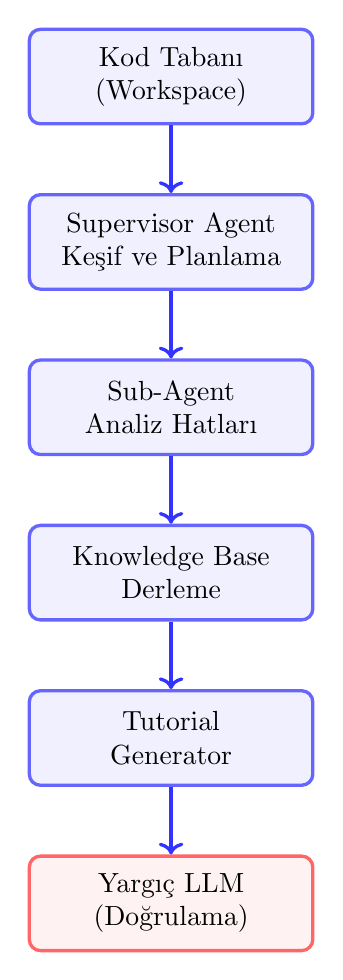
\begin{tikzpicture}[
        box/.style={rounded corners, draw=blue!60, fill=blue!6, very thick, minimum width=36mm, minimum height=12mm, align=center},
        flow/.style={->, very thick, draw=blue!80}
    ]
        \node[box] (input) at (0,0) {Kod Tabanı\\(Workspace)};
        \node[box] (analysis) at (0,-2.1) {Supervisor Agent\\Keşif ve Planlama};
        \node[box] (subpipe) at (0,-4.2) {Sub-Agent\\Analiz Hatları};
        \node[box] (kb) at (0,-6.3) {Knowledge Base\\Derleme};
        \node[box] (tutorial) at (0,-8.4) {Tutorial\\Generator};
        \node[box, fill=red!5, draw=red!60] (judge) at (0,-10.5) {Yargıç LLM\\(Doğrulama)};

        \draw[flow] (input) -- (analysis);
        \draw[flow] (analysis) -- (subpipe);
        \draw[flow] (subpipe) -- (kb);
        \draw[flow] (kb) -- (tutorial);
        \draw[flow] (tutorial) -- (judge);
    \end{tikzpicture}
    \caption{Bilgi üretim hattının üst düzey görünümü.}
    \label{fig:pipeline-overview}
\end{figure}

Mimari, iki aşamalı Sub-Agent kurgusu üzerine kuruludur. Supervisor Agent keşif, planlama ve orkestrasyon görevlerini yürütür; bağlam yükünü azaltmak için işleri Sub-Agent'lara devreder. Sub-Agent'lar kendi çalışma alanlarında ayrık olarak analiz yapar, bulgularını kalıcı depolara kaydeder ve Supervisor Agent’a raporlar. Supervisor Agent bu çıktıları birleştirerek nihai Knowledge Base'i oluşturur; ardından içerik üretimi için Tutorial Generator bileşenini tetikler.

Deterministik görev bölme yaklaşımıyla kaynak dosya altındaki ilk seviye klasörler ayrı Sub-Agent'lara atanır. Alternatif olarak Supervisor Agent, planlama parametreleri ve bir yapılacaklar listesi üzerinden görevleri dinamik biçimde güncelleyebilir. Sub-Agent'ların kod tabanına yalnızca okuma, kendi çalışma alanlarına ise yazma yetkisi vardır; böylece bağlam yönetimi ve çıktı doğrulaması sadeleşir.

\begin{figure}[htbp]
    \centering
    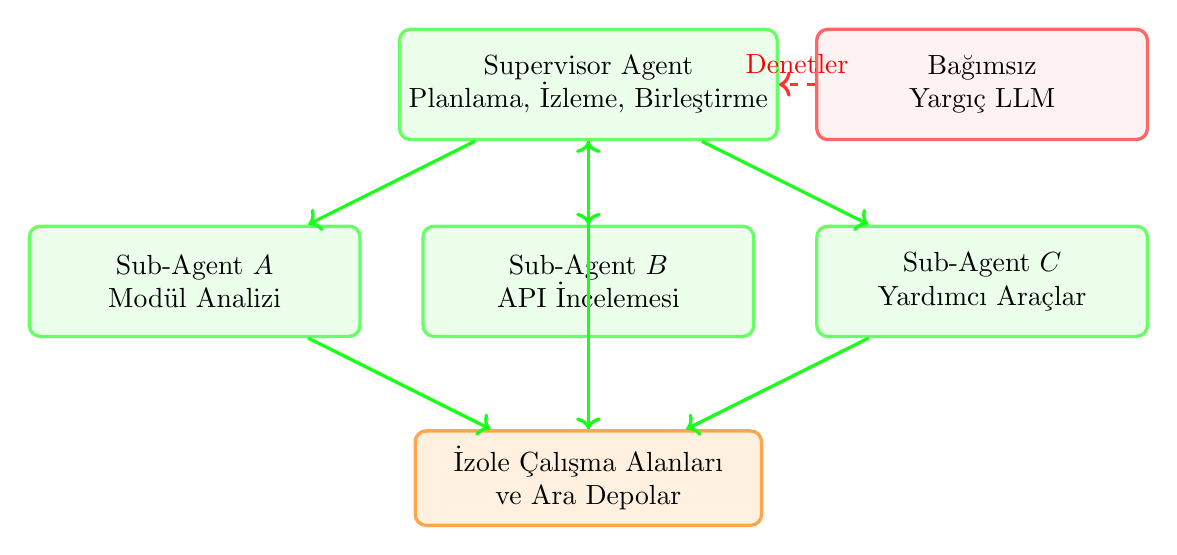
\begin{tikzpicture}[
        layer/.style={rounded corners, draw=green!60, fill=green!8, very thick, minimum width=42mm, minimum height=14mm, align=center},
        datastore/.style={rounded corners, draw=orange!70, fill=orange!12, very thick, minimum width=44mm, minimum height=12mm, align=center},
        flow/.style={->, very thick, draw=green!90}
    ]
        \node[layer] (main) at (7,4) {Supervisor Agent\\Planlama, İzleme, Birleştirme};
        \node[layer] (sub1) at (2,1.5) {Sub-Agent $A$\\Modül Analizi};
        \node[layer] (sub2) at (7,1.5) {Sub-Agent $B$\\API İncelemesi};
        \node[layer] (sub3) at (12,1.5) {Sub-Agent $C$\\Yardımcı Araçlar};
        \node[datastore] (stores) at (7,-1) {İzole Çalışma Alanları\\ve Ara Depolar};
        \node[layer, fill=red!5, draw=red!60] (judge) at (12, 4) {Bağımsız\\Yargıç LLM};

        \draw[flow] (main) -- (sub1);
        \draw[flow] (main) -- (sub2);
        \draw[flow] (main) -- (sub3);
        \draw[flow] (sub1) -- (stores);
        \draw[flow] (sub2) -- (stores);
        \draw[flow] (sub3) -- (stores);
        \draw[flow] (stores) -- (main);
        \draw[flow, dashed, draw=red!80] (judge) -- node[above, text=red]{Denetler} (main);
    \end{tikzpicture}
    \label{fig:agent-architecture}
\end{figure}


\noindent\textbf{Başarı Kriterleri ve Metrikler.}
Sistemin başarısı, teorik formüller yerine, sistem bileşenleri tarafından toplanan operasyonel veriler ve Yargıç LLM tarafından gerçekleştirilen kalite ölçümleri ile değerlendirilir.

\begin{itemize}
    \item \textbf{Operasyonel Verimlilik (Efficiency):} Sistemin bir projeyi analiz etme maliyeti şu üç temel metrikle izlenir:
    \begin{itemize}
        \item \textit{Token Tüketimi:} Toplam Girdi/Çıktı token sayısı (Maliyet analizi için).
        \item \textit{Süre (Duration):} Knowledge Base ve Tutorial fazlarının tamamlanma süreleri.
        \item \textit{Araç Kullanımı (Tool Calls):} Ajanların dosya okuma ve yazma sıklığı.
    \end{itemize}

    \item \textbf{İçerik Kalitesi (Yargıç LLM):} Üretilen eğitim içeriklerinin kalitesi, bağımsız bir LLM (Yargıç) tarafından 1-5 ölçeğinde puanlanır. Temel kriterler şunlardır:
    \begin{itemize}
        \item \textit{Doğruluk (Accuracy):} Kod örneklerinin gerçek kaynak kodla uyumu.
        \item \textit{Tamamlayıcılık (Completeness):} Konunun ne kadar kapsandığı.
        \item \textit{Pedagoji:} Anlatım sırasının mantıksal akışı.
    \end{itemize}

    \item \textbf{Süreç Dayanıklılığı (Robustness):}
    \begin{itemize}
        \item \textit{Bağlam Taşması (Context Overflow):} LLM'in hafıza sınırını aşma olaylarının sayısı.
        \item \textit{Toparlanma Başarısı:} Hata sonrası `retry` mekanizmasının başarı oranı.
    \end{itemize}
\end{itemize}


\section{Gereksinim Analizi}
\label{sec:gereksinim-analizi}

Gereksinimler üç düzeyde sınıflandırılmıştır: kullanıcı rolleri, sistem modülleri ve işlevsel akış. Sistemin iki temel kullanıcısı bulunmaktadır. Birincisi, Bilgi Bankası ve eğitim çıktıları üzerinden kod tabanını öğrenen geliştiricidir. İkincisi ise ajan süreçlerini başlatan, izleyen ve üretilen çıktının bütünlüğünü doğrulayan sistem operatörüdür. 

Sistem modülleri dört ana bileşenden oluşur. Supervisor Agent; keşif, planlama, görev dağıtımı ve Sub-Agent'lardan gelen çıktıları birleştirme görevlerini üstlenen merkezî unsurdur. Sub-Agent'lar; deterministik olarak veya koşula bağlı şekilde üretilen, belirli dizinleri veya görev kümelerini analiz eden ve izole çalışma alanlarında faaliyet gösteren ajanlardır. Knowledge Base deposu, tüm Sub-Agent özetlerinin toplandığı yapısal bir klasör düzeni sunarken, Tutorial Generator bileşeni bu Knowledge Base’i kullanarak pedagojik değer taşıyan eğitim materyallerini bağımsız bir çıktı klasörü altında üretir.

Sistemin işlevsel akışı ardışık beş aşamada gerçekleşir. İlk aşamada Supervisor Agent kod tabanının dosya yapısını çıkarır, kritik bileşenleri analiz eder ve deterministik ya da dinamik olarak görev listesini oluşturur. İkinci aşamada bu görevler ilgili Sub-Agent'lara dağıtılır. Üçüncü aşamada Sub-Agent'lar, sorumlu oldukları kod parçalarını inceleyerek özetlerini kendi çalışma dizinlerine kaydeder. Dördüncü aşamada Supervisor Agent bu alt çıktıları bir araya getirerek bütünleşik Knowledge Base’i oluşturur ve kalite kontrolünü gerçekleştirir. Son aşamada Tutorial Generator, oluşturulan bu Knowledge Base’i geliştiricilerin kolay öğrenebileceği bir pedagojik formata dönüştürür.

İşlevsel olmayan gereksinimler ise sistemin güvenlik, izlenebilirlik, genişletilebilirlik ve performans özelliklerini belirlemektedir. Sistem, özellikle dizin gezintisi (path traversal) zafiyetlerine karşı güvenli olacak şekilde tasarlanmalı; tüm API anahtarları gizli tutulmalı ve kod tabanına gömülmemelidir. Ayrıca ajanların karar verme süreçleri, özellikle görev delegasyonu  ve dosya işlemleri Phoenix aracı üzerinden ayrıntılı biçimde loglanmalıdır. Mimari, yeni araçların veya ajan türlerinin eklenmesine açık bir genişletilebilirlik sunmalıdır. Son olarak performans açısından, bir prototip olması nedeniyle süreç karmaşıklığını azaltmak amacıyla Sub-Agent'ların paralel değil, sıralı olarak çalıştırılması tercih edilmiştir.

\section{Fizibilite}
\label{sec:fizibilite}

\subsection{Teknik Fizibilite}
\label{sec:teknik-fizibilite}

\subsubsection{Donanım}
\label{sec:donanim-fizibilitesi}
Model eğitimi hedeflenmediği için yüksek donanım yatırımı gerekmez. LLM çağrıları API tabanlıdır; standart bir geliştirici bilgisayarı yeterlidir. İş yükü Sub-Agent'lara bölündüğü için bellek baskısı artmaz, uzun dosya okumaları engellenir.

\subsubsection{Yazılım}
\label{sec:yazilim-fizibilitesi}
\begin{itemize}
    \item \textbf{İşletim Sistemi:} Windows, macOS veya Linux.
    \item \textbf{Programlama Dili:} Python 3.10+ (Backend), TypeScript/React (Frontend).
    \item \textbf{Çerçeveler ve Araçlar:} \texttt{smolagents} (Ajan Orkestrasyonu), \texttt{LiteLLM} (AI Gateway), \texttt{Next.js} (Web Arayüzü), \texttt{Phoenix} (İzleme).
\end{itemize}

\subsection{Yasal Fizibilite}
\label{sec:yasal-fizibilite}
Kullanılan kütüphaneler MIT veya Apache~2.0 benzeri açık kaynak lisanslarıyla dağıtılır. Analiz edilecek kod tabanının proje ekibine ait olması veya lisans uyumunun sağlanması yeterlidir.

\subsection{Ekonomik Fizibilite}
\label{sec:ekonomik-fizibilitesi}

Projenin ekonomik fizibilitesi, düşük başlangıç maliyeti ve yüksek katma değer üretme potansiyeli sayesinde olumlu olarak değerlendirilmektedir. Sistem, büyük ölçüde açık kaynaklı yazılımlar ve bulut tabanlı LLM servisleri üzerine kurulu olup, merkezi ve sürekli bir altyapı yatırımı gerektirmemektedir.

\subsubsection{Giderler}

Temel bileşenler ücretsizdir. Maliyet kalemleri ağırlıklı olarak mühendislik eforu ve LLM API çağrılarından oluşmaktadır. Geliştirme ve test aşamalarında Google AI Studio veya OpenRouter üzerinden sunulan ücretsiz ya da düşük maliyetli modeller kullanılabilmektedir. Son kullanıcıya sunulan nihai dokümantasyon ve eğitim içeriklerinin üretiminde ise daha güçlü modeller tercih edilerek kalite–maliyet dengesi sağlanmaktadır.

Başlıca gider kalemleri aşağıda özetlenmiştir:

\begin{itemize}
    \item \textbf{Geliştirme Maliyeti:} Sistem mimarisi, çoklu ajan orkestrasyonu ve prompt mühendisliği için harcanan mühendislik eforu.
    \item \textbf{LLM API Maliyetleri:}
    \begin{itemize}
        \item \textit{Gemini 2.5 Pro:} Ortalama bir proje analizi için yaklaşık \$0.10 – \$0.50.
        \item \textit{GPT-OSS-120B:} Yüksek kalite gerektiren son tutorial üretimi aşamalarında sınırlı ve seçici kullanım.
    \end{itemize}
\end{itemize}

\subsubsection{Katma Değer}

Sistemin sağladığı katma değer, doğrudan parasal kazançtan ziyade zaman tasarrufu ve verimlilik artışı üzerinden ortaya çıkmaktadır. Bu bağlamda öne çıkan kazanımlar şunlardır:

\begin{itemize}
    \item Dokümantasyon ve proje öğrenme süreçlerinde \%80’den fazla zaman tasarrufu.
    \item Yeni geliştiricilerin projeye adaptasyon süresinin önemli ölçüde kısalması (hızlı onboarding).
    \item Kod tabanı değiştikçe ajanların yeniden çalıştırılmasıyla sürekli güncel dokümantasyon elde edilmesi.
    \item İlk kullanımda elde edilen zaman kazancı sayesinde sistemin kendi maliyetini kısa sürede amorti edebilmesi.
\end{itemize}

Bu yönleriyle proje, hem bireysel geliştiriciler hem de kurumsal yazılım ekipleri için ekonomik açıdan sürdürülebilir ve ölçeklenebilir bir çözüm sunmaktadır.

\subsection{İşgücü ve Zaman Fizibilitesi}
\label{sec:isgucu-zaman-fizibilitesi}

\textbf{Ekip:} 2 kişi (yazılım/araştırma odaklı).

\textbf{Genel Yaklaşım:} İlk sürüm için 8–12 hafta aralığında bir geliştirme süresi öngörülür. Detaylı şema şekil 2.2'de sunulmuştur.

\begin{figure}[H]
\centering
\begin{ganttchart}[
    hgrid,
    vgrid,
    x unit=0.45cm,
    y unit chart=0.6cm,
    bar height=0.45,
    bar label font=\scriptsize,
    bar/.append style={fill=gray!30},
]{1}{12}          % ← Haftalar (1–12)
    
    \gantttitle{İşgücü Gantt Şeması (12 Hafta)}{12} \\

    % Geliştirici
    \ganttgroup{Geliştirici}{1}{12} \\
    \ganttbar{Repo + Dosya Katmanı}{1}{2} \\
    \ganttbar{Sub-Agent Temelleri}{3}{4} \\
    \ganttbar{Loglama + Retry}{9}{10} \\

    % Araştırmacı
    \ganttgroup{Araştırmacı}{1}{12} \\
    \ganttbar{Knowledge Base + Şablonlar}{5}{6} \\
    \ganttbar{Eğitim Pipeline Tasarımı}{7}{8} \\

    % Ortak Görevler
    \ganttgroup{Ortak Görevler}{1}{12} \\
    \ganttbar{Sub-Agent Tasarım Konsepti}{3}{4} \\
    \ganttbar{E2E Test + Raporlama}{11}{12} \\

\end{ganttchart}
\caption{İşgücü Fizibilitesi – Rol Bazlı Gantt Şeması}
\end{figure}


\chapter{SİSTEM TASARIMI}
\label{ch:sistem-tasarimi}

Bu bölümde, geliştirilen çok ajanlı yapay zekâ analiz platformunun sistem tasarımı detaylandırılmaktadır. Tasarım mimarisi; kullanıcı etkileşimi, veri yönetimi ve nesne yönelimli modelleme olmak üzere üç temel eksende kurgulanmıştır. Amaç, karmaşık yazılım projelerini otonom olarak analiz edebilen ve eğitsel içerik üretebilen modüler, güvenli ve ölçeklenebilir bir yapı sunmaktır.

%---------------------------------------------------------
\section{Arayüz Tasarımı}
\label{sec:arayuz-tasarimi}

Sistem, kullanım kolaylığı ve operasyonel esnekliği bir arada sunmak amacıyla ikili bir arayüz yapısı benimsemiştir: Operasyonel süreçler için **Komut Satırı Arayüzü (CLI)** ve analitik çıktılar için **Web Tabanlı Kontrol Paneli**.

\subsection{Komut Satırı Arayüzü (CLI)}
Analiz süreçlerinin başlatılması ve yönetilmesi, geliştiricilerin alışkın olduğu terminal ortamı üzerinden gerçekleştirilir. Kullanıcılar, tek bir komut ile hedef projeyi sisteme tanıtır ve analiz sürecini başlatır. Sistemin CLI katmanı, arka planda çalışan yapay zekâ ajanlarının durumunu, kaynak tüketimini ve ilerleme yüzdelerini anlık olarak terminal ekranına yansıtır. Bu yalın tasarım, sistemin CI/CD (Sürekli Entegrasyon/Dağıtım) boru hatlarına kolayca entegre edilmesine olanak tanır.

\subsection{Web Tabanlı Kontrol Paneli (Web Dashboard)}
Otonom analiz tamamlandıktan sonra üretilen Knowledge Base ve eğitim materyallerinin son kullanıcıya sunulması için modern web teknolojileri (Next.js ve React) kullanılarak geliştirilmiş bir arayüz mevcuttur. Bu panelin temel işlevleri şunlardır:

\begin{itemize}
    \item **Proje Kütüphanesi:** Analiz edilen farklı kod tabanlarının görsel kartlar halinde listelenmesi ve yönetilmesi.
    \item **Etkileşimli İçerik Görüntüleyici:** Ajanlar tarafından üretilen Markdown formatındaki ders içeriklerinin, kod renklendirme (syntax highlighting) ve dinamik diyagram destekli olarak okunabilir hale getirilmesi.
    \item **Akıllı Gezinme:** Oluşturulan müfredat içerikleri arasında hiyerarşik geçiş imkanı.
\end{itemize}

Şekil~\ref{fig:ui-flow}'te sistemin operasyonel ve analitik arayüzleri arasındaki veri akış diyagramı sunulmuştur.

\begin{figure}[H]
    \centering
    \resizebox{0.95\textwidth}{!}{%
    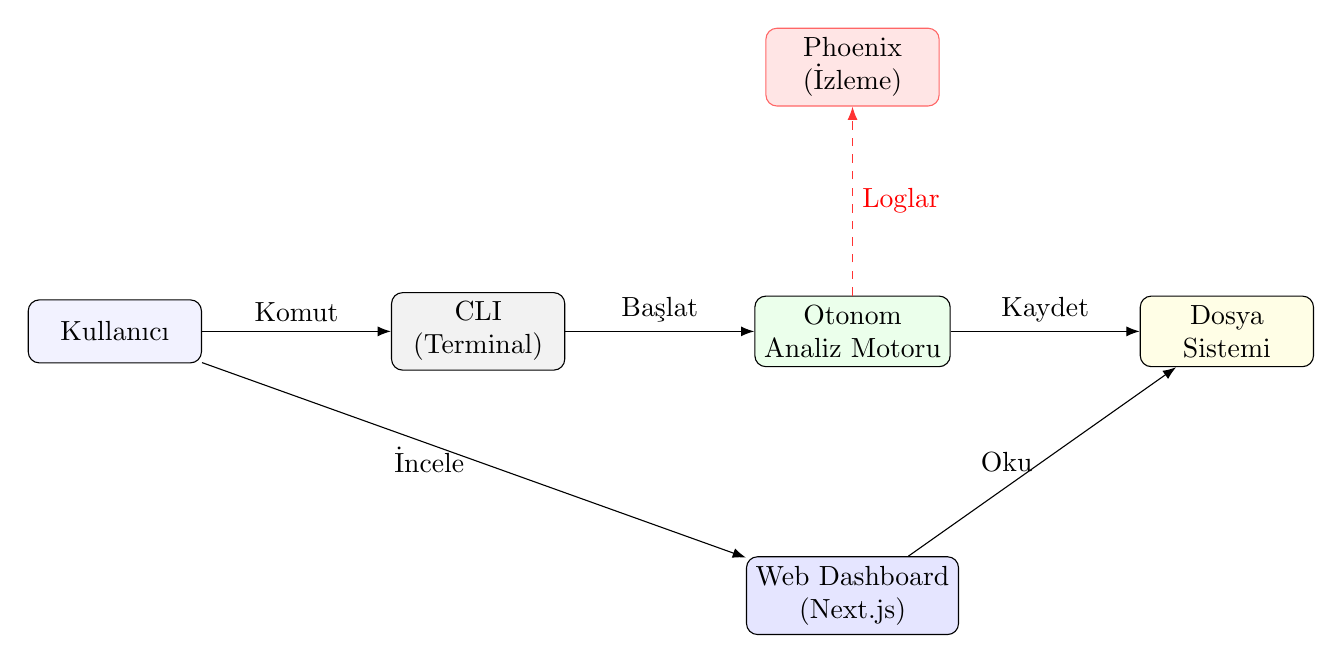
\begin{tikzpicture}[
        node distance=2.4cm,
        >=Latex,
        box/.style={
            draw,
            rounded corners,
            minimum width=22mm,
            minimum height=8mm,
            align=center,
            fill=blue!5
        }
    ]
        \node[box] (user) {Kullanıcı};
        \node[box, right=of user, fill=gray!10] (cli) {CLI\\(Terminal)};
        \node[box, right=of cli, fill=green!8] (pipeline) {Otonom\\Analiz Motoru};
        \node[box, above=of pipeline, fill=red!10, draw=red!60] (phoenix) {Phoenix\\(İzleme)};
        \node[box, right=of pipeline, fill=yellow!10] (fs) {Dosya\\Sistemi};
        \node[box, below=of pipeline, fill=blue!10] (web) {Web Dashboard\\(Next.js)};

        \draw[->] (user) -- node[above]{Komut} (cli);
        \draw[->] (cli) -- node[above]{Başlat} (pipeline);
        \draw[->] (pipeline) -- node[above]{Kaydet} (fs);
        \draw[->] (web) -- node[left]{Oku} (fs);
        \draw[->] (user) -- node[left]{İncele} (web);
        \draw[dashed, ->, draw=red!80] (pipeline) -- node[right, text=red]{Loglar} (phoenix);
    \end{tikzpicture}%
    }
    \caption{Kullanıcı etkileşimi ve veri akış şeması.}
    \label{fig:ui-flow}
\end{figure}

%---------------------------------------------------------
\section{Veri Yapısı Tasarımı}
\label{sec:veri-yapisi-tasarimi}

Proje mimarisinde, karmaşık veritabanı yönetim sistemleri yerine, taşınabilirlik ve şeffaflığı ön planda tutan, dosya sistemi tabanlı (filesystem-based) bir veri yaklaşımı tercih edilmiştir. Bu tasarım kararı, üretilen dokümantasyonun versiyon kontrol sistemleri (örn. Git) ile uyumlu olmasını ve projenin kendisiyle birlikte saklanabilmesini sağlar.

\subsection{Yapılandırma Yönetimi}
Sistemin davranış kalıpları ve parametreleri, merkezi yapılandırma dosyaları üzerinden yönetilir. Model seçimleri, API erişim anahtarları ve global sistem ayarları tek bir noktadan kontrol edilirken, web arayüzünde görüntülenecek metadata bilgileri ayrıştırılmış formatlarda saklanır.

\subsection{İzole Çalışma Alanları (Scoped Filesystem)}
Veri güvenliğini sağlamak ve projeler arası çakışmaları önlemek adına "İzole Dosya Sistemi" mimarisi uygulanmıştır. Her analiz süreci, kendine tahsis edilen üç katmanlı bir dizin yapısı içinde çalışır:

\begin{enumerate}
    \item **Kaynak Katmanı (Okuma):** Ajanların sadece okuma iznine sahip olduğu, orijinal kod tabanının bulunduğu güvenli alan.
    \item **Bellek Katmanı (Geçici):** Analiz sürecinde oluşturulan ara özetlerin ve notların tutulduğu çalışma alanı.
    \item **Çıktı Katmanı (Yazma):** Nihai eğitim materyallerinin ve raporların derlendiği sonuç klasörü.
\end{enumerate}

Bu yapı sayesinde, yapay zekâ ajanlarının proje dosyalarına zarar vermesi engellenmiş ve veri bütünlüğü garanti altına alınmıştır.

%---------------------------------------------------------
\section{Nesneye Yönelik Tasarım ve Ajan Mimarisi}
\label{sec:ajan-mimarisi}

Sistemin yazılım mimarisi, klasik statik sınıf hiyerarşileri yerine, esnekliği maksimize eden **Bileşimsel (Composition-based)** ve **Dinamik** bir tasarım modeline dayanır. Ajanlar, sabit kod blokları olarak değil, çalışma zamanında (runtime) ihtiyaca göre bir araya getirilen yetenek kümeleri olarak kurgulanmıştır.

\subsection{Dinamik Ajan Yapısı}
Platform içerisindeki her bir ajan (Supervisor Agent, Sub-Agent, Tutorial Generator), üç temel bileşenin dinamik birleşimiyle oluşturulur:

\begin{itemize}
    \item **Kimlik ve Rol Tanımı (Prompt):** Ajanın amacını, kurallarını ve davranış biçimini belirleyen doğal dil talimatlarıdır.
    \item **Yetenek Seti (Toolkit):** Ajanın dosya okuma, komut çalıştırma veya internette arama yapma gibi teknik becerilerini tanımlayan modüler fonksiyon kütüphaneleridir.
    \item **Dil Modeli (LLM):** Görevin karmaşıklığına göre seçilen, ajana zeka sağlayan işlem birimidir.
\end{itemize}

Bu modüler yapı, sisteme yeni yeteneklerin eklenmesini veya ajan davranışlarının değiştirilmesini, kaynak kodda köklü değişiklikler yapmadan mümkün kılar.

\subsection{Orkestrasyon Katmanı}
Ajanların koordinasyonu ve görev dağılımı, üst seviye yönetici sınıflar tarafından sağlanır. Sistemde ana yönetici rolünü üstlenen bu yapı, analiz sürecini mantıksal aşamalara (Bilgi Toplama, Planlama, İçerik Üretimi) böler ve her aşama için gerekli ajanları senkronize bir şekilde devreye sokar.

Şekil~\ref{fig:class-diagram}'de sistemin dinamik nesne mimarisi özetlenmiştir.

\begin{figure}[H]
    \centering
    \resizebox{0.85\textwidth}{!}{%
    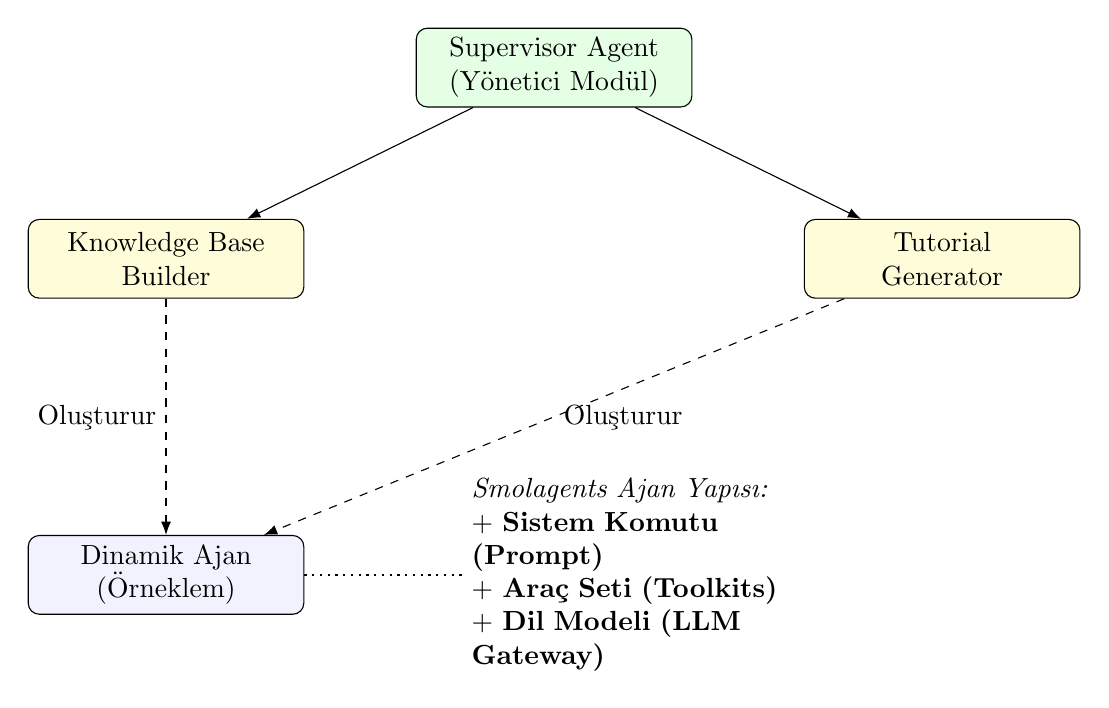
\begin{tikzpicture}[
        node distance=2.0cm,
        >=Latex,
        class/.style={
            draw,
            rounded corners,
            minimum width=35mm,
            minimum height=10mm,
            align=center,
            fill=blue!5
        }
    ]
        \node[class, fill=green!10] (orch) {Supervisor Agent\\(Yönetici Modül)};
        \node[class, below left=of orch, fill=yellow!15] (kb) {Knowledge Base\\Builder};
        \node[class, below right=of orch, fill=yellow!15] (tut) {Tutorial\\Generator};
        \node[class, below=of kb, yshift=-1cm] (agents) {Dinamik Ajan\\(Örneklem)};

        \draw[->] (orch) -- (kb);
        \draw[->] (orch) -- (tut);
        \draw[->, dashed] (kb) -- node[left]{Oluşturur} (agents);
        \draw[->, dashed] (tut) -- node[right]{Oluşturur} (agents);
        
        \node[right=of agents, text width=4.5cm, align=left] (components) {
            \textit{Smolagents Ajan Yapısı:}\\
            + \textbf{Sistem Komutu (Prompt)}\\
            + \textbf{Araç Seti (Toolkits)}\\
            + \textbf{Dil Modeli (LLM Gateway)}
        };
        \draw[dotted, thick] (agents) -- (components);
    \end{tikzpicture}%
    }
    \caption{Orkestrasyon yapısı ve dinamik ajan üretimi.}
    \label{fig:class-diagram}
\end{figure}

Bu mimari tercih, sistemin bakım maliyetini düşürmekte ve farklı programlama dilleri veya teknolojiler için kolayca özelleştirilebilmesine olanak tanımaktadır.
\chapter{UYGULAMA SONUÇLARI ve TESTLER}
\label{ch:uygulama-sonuclari}

\section{Uygulama Tanıtımı}
\label{sec:uygulama-tanitimi}

Geliştirilen sistem, son kullanıcıların karmaşık komut dizileriyle uğraşmadan, doğrudan doğal dil ve basit terminal konfigürasyonlarıyla çalıştırabileceği bir yapı sunmaktadır. Uygulama, ana dizinde bulunan çalıştırıcı betik üzerinden yönetilmektedir. Bu betik, gerekli ortam değişkenlerini yükler, sanal ortamı kontrol eder ve Python tabanlı komut satırı arayüzünü başlatır.

Kullanıcılar için iki temel çalışma modu tasarlanmıştır:
\begin{enumerate}
    \item \textbf{Deep Agent Modu:} Sub-Agent mimarisinin tam kapasiteyle çalıştığı, önce Knowledge Base oluşturup ardından eğitim içeriği üreten mod.
    \item \textbf{Baseline Modu:} Karşılaştırma amacıyla geliştirilen, Sub-Agent ve Knowledge Base kullanmadan doğrudan tek bir ajanın (ReAct mimarisi) tüm işi yapmaya çalıştığı mod.
\end{enumerate}

Sistem, otonom analiz ve içerik üretimi için yapılandırılmış komut setleri ile çalıştırılmaktadır. Kullanıcı, hedef kod tabanının yolunu belirterek analizi başlatabilir; karşılaştırma amaçlı olarak sistemin alt-ajan kullanmadan doğrudan tekil bir yapı üzerinden ilerlediği bir temel (baseline) modu da desteklenmektedir.

Uygulama çalıştığında, arka planda olay tabanlı bir loglama sistemi devreye girer. Kullanıcı terminalde anlık ilerlemeyi (ajanın o an hangi dosyayı okuduğu, hangi kararı verdiği) görebilirken, üretilen Markdown formatındaki eğitim dokümanları ve analiz raporları ilgili dizin altında otomatik olarak oluşturulur.

\section{Test Sonuçları}
\label{sec:test-sonuclari}

Sistemin başarımı, \textit{Sistem Analizi} bölümünde belirlenen gereksinimler doğrultusunda, özellikle maliyet etkinliği ve bağlam (context) yönetimi açısından test edilmiştir. Bu testlerde "Agent Lightning" kütüphanesi örnek proje olarak kullanılmış ve aynı donanım/ortam şartlarında hem Baseline hem de Deep Agent modları çalıştırılmıştır.

Elde edilen veriler, sistemin işlem yükü, token tüketimi ve araç kullanım sıklığı gibi performans metriklerini ortaya koymaktadır.

\subsection{Maliyet ve Bağlam Analizi (Deney 4)}

Büyük Dil Modelleri ile çalışan sistemlerde en kritik darboğaz, modelin bağlam penceresi ve token başına maliyettir. Aşağıdaki Tablo \ref{tab:cost-context}, Baseline ve Deep Agent yaklaşımlarının "Tutorial Üretim Fazı" için karşılaştırmalı performansını göstermektedir.

\begin{table}[htbp]
    \centering
    \caption{Baseline ve Deep Agent Modellerinin Tutorial Üretim Fazı Karşılaştırması}
    \label{tab:cost-context}
    \begin{tabular}{|l|c|c|}
        \hline
        \textbf{Metrik} & \textbf{Baseline Agent} & \textbf{Deep Agent} \\
        \hline
        Toplam Süre (saniye) & 378.25 & 620.98 \\
        \hline
        Girdi Token Sayısı (Input) & 1,732,968 & 3,236,280 \\
        \hline
        Çıktı Token Sayısı (Output) & 77,745 & 145,053 \\
        \hline
        Toplam Token Maliyeti & \textbf{1.81 Milyon} & \textbf{3.38 Milyon} \\
        \hline
        Araç Çağrı Sayısı (Tool Calls) & 32 & 43 \\
        \hline
        Bağlam Taşması (Overflow) & 0 & 0 \\
        \hline
    \end{tabular}
\end{table}

\noindent\textbf{Analiz:}
Tablo incelendiğinde, Deep Agent mimarisinin Baseline'a göre yaklaşık iki kat daha fazla token tükettiği ve işlemin daha uzun sürdüğü görülmektedir. İlk bakışta bu bir dezavantaj gibi görünse de, çıktının kalitesi ve derinliği göz önüne alındığında (Bkz. Bölüm \ref{sec:dogrulama}), bu "fazladan" maliyetin sisteme \textbf{bağlam zenginliği} olarak geri döndüğü anlaşılmaktadır. Baseline ajan, daha az token harcamasına rağmen yüzeysel ve genel geçer çıktılar üretirken; Deep Agent, oluşturduğu Knowledge Base'i bağlamına yüklediği için (input token artışı buradan kaynaklanmaktadır) çok daha detaylı, kod referanslı ve teknik doğruluğu yüksek içerikler üretmiştir.

Ayrıca, her iki sistemde de "Bağlam Taşması (Context Overflow)" olayının "0" olması, geliştirilen hız sınırlamalı dil modeli sarmalayıcısının ve token yönetim mekanizmasının başarılı bir şekilde çalıştığını kanıtlamaktadır.

\section{Doğrulama}
\label{sec:dogrulama}

Sistemin ürettiği çıktıların kalitesi ve kullanıcı gereksinimlerini karşılama düzeyi, güncel bir yöntem olan "Judge LLM" (Yargıç LLM) metodu ile doğrulanmıştır.

\subsection{Yargıç LLM Değerlendirmesi (Deney 2)}

Bu deneyde, SOTA (State-of-the-Art) kabul edilen \textbf{Claude 4.5 Sonnet} ve \textbf{GPT-OSS-120B} modelleri "tarafsız yargıç" olarak atanmıştır. Yargıçlara, hem Baseline (Seri A) hem de Deep Agent (Seri B) tarafından üretilen eğitim dokümanları, kaynak kod ile birlikte verilmiş ve şu üç kriterde puanlama yapmaları istenmiştir:

\begin{enumerate}
    \item \textbf{Doğruluk (Fidelity):} Üretilen kod örnekleri ve açıklamalar gerçek kod tabanıyla örtüşüyor mu? Halüsinasyon var mı?
    \item \textbf{Pedagoji (Pedagogy):} Anlatım, bir öğrencinin anlayabileceği şekilde basitten zora doğru mu? Örnekler öğretici mi?
    \item \textbf{Kapsam (Coverage):} Kod tabanının kritik özelliklerine değinilmiş mi yoksa sadece yüzeyde mi kalınmış?
\end{enumerate}

Yargıçların değerlendirme sonuçları Tablo \ref{tab:win-rate}’de özetlenmiştir.

\begin{table}[htbp]
    \centering
    \caption{Yargıç LLM'lerin Kalite Değerlendirmesi (5 üzerinden puan)}
    \label{tab:win-rate}
    \begin{tabular}{|l|c|c|c|c|c|c|}
        \hline
        \multirow{2}{*}{\textbf{Yargıç Model}} & \multicolumn{2}{c|}{\textbf{Doğruluk}} & \multicolumn{2}{c|}{\textbf{Pedagoji}} & \multicolumn{2}{c|}{\textbf{Kapsam}} \\
        \cline{2-7}
         & Base & \textbf{Deep} & Base & \textbf{Deep} & Base & \textbf{Deep} \\
        \hline
        Claude 4.5 Sonnet & 3 & \textbf{5} & 3 & \textbf{5} & 3 & \textbf{5} \\
        \hline
        GPT-OSS-120B & 4 & \textbf{5} & 4 & \textbf{5} & 4 & \textbf{5} \\
        \hline
    \end{tabular}
\end{table}

\begin{figure}[H]
    \centering
    \begin{tikzpicture}[scale=0.9]
        \begin{axis}[
            ybar,
            enlarge x limits=0.25,
            legend style={at={(0.5,-0.2)}, anchor=north, legend columns=-1},
            ylabel={Puan (1-5)},
            symbolic x coords={Doğruluk, Pedagoji, Kapsam},
            xtick=data,
            nodes near coords,
            nodes near coords align={vertical},
            ylimits={0,6},
            bar width=15pt,
            width=10cm,
            height=6cm,
            title={Ortalama Yargıç Değerlendirme Puanları}
        ]
            \addplot[fill=gray!40] coordinates {(Doğruluk,3.5) (Pedagoji,3.5) (Kapsam,3.5)};
            \addplot[fill=blue!40] coordinates {(Doğruluk,5.0) (Pedagoji,5.0) (Kapsam,5.0)};
            \legend{Baseline Agent, Deep Agent}
        \end{axis}
    \end{tikzpicture}
    \caption{Baseline ve Deep Agent modellerinin kalite metrikleri bazında karşılaştırılması.}
    \label{fig:evaluation-comparison}
\end{figure}

\noindent\textbf{Sonuç Yorumu:}
Her iki yargıç modeli de **Deep Agent (Seri B)** tarafından üretilen dokümanları "açık ara kazanan" (Winner: B) olarak ilan etmiştir.
\begin{itemize}
    \item \textbf{Doğruluk:} Baseline modelin, kullanılmayan (deprecated) API'leri önerdiği veya sınıf isimlerini yanlış yazdığı tespit edilmiştir. Deep Agent ise Knowledge Base'den doğrulama yaptığı için \%100'e yakın doğruluk sağlamıştır.
    \item \textbf{Pedagoji:} Deep Agent; "Hello World" örneğinden başlayıp, ileri seviye konulara (Distributed Training, Async Execution) doğru giden yapılandırılmış bir müfredat sunmuştur. Baseline ise konuları kopuk parçalar halinde sunmuştur.
\end{itemize}

\subsection{Gereksinim Uyumluluk Analizi}

Projenin başlangıcında (Bkz. Bölüm \ref{sec:gereksinim-analizi}) belirlenen işlevsel ve işlevsel olmayan gereksinimlerin karşılanma durumu yapılan son denetimlerle (audit) doğrulanmıştır.

\begin{itemize}
    \item \textbf{Sub-Agent Mimarisi:} \checkmark Tamamlandı. Supervisor Agent dinamik olarak Sub-Agent'lar oluşturabilmekte ve izole çalışma alanlarını yönetebilmektedir.
    \item \textbf{Güvenlik (Path Traversal):} \checkmark Tamamlandı. Geliştirilen kısıtlanmış dosya erişim modülü, ajanların sadece izin verilen dizinlere erişmesini garanti altına almıştır.
    \item \textbf{Knowledge Base Üretimi:} \checkmark Tamamlandı. Kod tabanından otomatik olarak kapsamlı bir Markdown Knowledge Base oluşturulabilmektedir.
    \item \textbf{Raporlama ve İzleme:} \checkmark Tamamlandı. Hem terminal çıktıları hem de JSON formatındaki metrik dosyaları ile süreç şeffaf hale getirilmiştir.
\end{itemize}

Bu sonuçlar, geliştirilen sistemin hedeflenen otonom eğitim içerik üretimi görevini başarıyla yerine getirdiğini ve Deep Agent mimarisinin, geleneksel yöntemlere göre kalite açısından belirgin bir üstünlük sağladığını doğrulamaktadır.

\chapter{SONUÇ VE TARTIŞMA}
\label{ch:sonuc-ve-tartisma}

Bu çalışmada, büyük ve karmaşık kod tabanlarını otomatize etmek amacıyla "Sub-Agent" mimarisine dayalı otonom bir yapay zekâ sistemi tasarlanmış ve prototipi geliştirilmiştir. Geliştirilen sistem, "Agent Lightning" gibi modern ve dokümantasyonu sınırlı kütüphaneler üzerinde test edilmiş; elde edilen sonuçlar hem nicel metrikler hem de nitel Yargıç LLM değerlendirmeleriyle analiz edilmiştir.

Proje kapsamında elde edilen temel sonuçlar ve tartışma başlıkları aşağıda sunulmuştur:

\section{Elde Edilen Kazanımlar}

\begin{enumerate}
    \item \textbf{Bağlam Sınırının Aşılması:} Geleneksel tek ajanlı sistemlerin en büyük problemi olan "bağlam penceresi" (context window) kısıtı, geliştirdiğimiz iki aşamalı (Knowledge Base Üretimi $\rightarrow$ İçerik Üretimi) mimari sayesinde aşılmıştır. Supervisor Agent'ın tüm dosyaları okumak yerine, görevi alt ajanlara dağıtması ve sadece özet bilgiyi (Knowledge Base) kullanması, sistemin binlerce dosyalık projelerde bile "bağlam taşması" yaşamadan çalışmasını sağlamıştır.

    \item \textbf{Kalite ve Derinlik Artışı:} Yapılan karşılaştırmalı testler (Bölüm \ref{sec:test-sonuclari}), Deep Agent stratejisinin token maliyetini artırmasına rağmen (Baseline: 1.8M vs Deep: 3.3M), çıktı kalitesinde tartışılmaz bir üstünlük sağladığını göstermiştir. Baseline ajan yüzeysel bilgiler verirken; Deep Agent, kodun derinliklerindeki mimari desenleri, asenkron çalışma yapılarını ve doğru sınıf isimlerini tespit ederek "kullanılabilir ve doğru" eğitim materyali üretmeyi başarmıştır. Yargıç LLM'ler, Deep Agent'a doğruluk ve pedagoji kriterlerinde tam puan (5/5) vermiştir.

    \item \textbf{Güvenli ve İzole Çalışma:} Tasarlanan kısıtlanmış dosya erişim modeli sayesinde, otonom ajanların sadece kendilerine atanan dizinlerde çalışması sağlanmış, böylece olası veri kaybı veya dizin gezintisi (path traversal) zafiyetleri mimari düzeyde engellenmiştir.
\end{enumerate}

\section{Kısıtlar ve Maliyet}

Sistemin sunduğu yüksek kalitenin bir bedeli olarak işlem süresi ve maliyeti artış göstermiştir. Deep Agent modunda bir kütüphanenin analizi ve tutorial üretimi ortalama 10-20 dakika sürmektedir. Bu süre, bir insanın haftalar süren öğrenme sürecine göre ihmal edilebilir olsa da, anlık yanıt bekleyen interaktif senaryolar için (örneğin IDE içi kod tamamlama) bu mimari şu an için yavaş kalabilir. Ayrıca token tüketiminin yüksek olması, GPT-OSS-120B gibi pahalı modellerle çalışıldığında maliyetli olabilir; bu nedenle sistemin Gemini 2.5 Pro veya açık kaynaklı (OSS) modellerle optimize edilmesi önerilmektedir.

\section{Gelecek Çalışmalar}

Mevcut prototipin başarısı, bu alanda yapılacak ileri çalışmalar için güçlü bir temel oluşturmaktadır. Gelecek dönemde şu geliştirmelerin yapılması hedeflenmektedir:

\begin{itemize}
    \item \textbf{İnsan Deneyleri:} Şu an Yargıç LLM'lerle yapılan doğrulamanın, gerçek yazılım geliştiriciler ve üniversite öğrencileriyle yapılacak A/B testleriyle (Deney 1 ve Deney 3) desteklenmesi.
    \item \textbf{Ablasyon Çalışmaları:} Bilgi Bankası bileşeninin etkisini daha net ölçmek için, sistemin farklı modüllerinin kapatılarak (ör. sadece RAG ile, Knowledge Base olmadan) test edilmesi (Deney 5).
    \item \textbf{Web Arayüzü:} Mevcut CLI yapısının, daha geniş kitlelere hitap edecek, sürükle-bırak özellikli bir Web UI ile zenginleştirilmesi.
\end{itemize}

Sonuç olarak, bu proje ile otonom ajanların sadece kod yazmakla kalmayıp, yazılan kodu "anlatma ve öğretme" konusunda da insan geliştiricilere güçlü bir asistan olabileceği kanıtlanmıştır.

\input {RD_projectChapters/6-chapter.tex}

\fi
\ifnum\projecttype=2
\chapter{GİRİŞ}
\label{ch:giris}

% --- 1.1 ---

\label{sec:ajan-mimari}

Modern yapay zeka uygulamalarının temelinde, devasa metin ve kod veri kümeleri üzerinde eğitilmiş Büyük Dil Modelleri (LLM) yer almaktadır. Bu modeller, kendilerine sunulan bilgiyi anlama ve üretme konusunda yüksek kapasiteye sahip olsalar da, tek başlarına karmaşık ve çok aşamalı görevleri yerine getirmede sınırlı kalmaktadır. Bu noktada ajan tabanlı sistemler devreye girmektedir. Bir ajan, LLM'yi karar alma çekirdeği olarak kullanır; hedefe yönelik planlama yapar, dosya okuma veya kod yürütme gibi yardımcı araçları etkinleştirir ve çevreden aldığı geri bildirime göre stratejisini günceller.

Örneğin finans teknolojileri alanında çalışan bir yazılım mühendisinin, on binlerce dosyadan oluşan yeni bir ödeme altyapısına katıldığını düşünelim. Geliştiricinin mimariyi anlaması, iş akışlarını kavraması ve basit bir değişikliği güvenle uygulayabilmesi çoğu zaman haftalar almaktadır. İnsan gözetiminde yürüyen bu uzun uyum sağlama süreci, kod tabanından yapılandırılmış bilgi çıkarabilen otonom sistemlerin yokluğunda daha da uzamakta; iş devri ve bakım maliyetleri yükselmektedir.

Bu mimarilerin en belirgin teknik kısıtlaması, LLM'lerin "bağlam penceresi" olarak bilinen veri işleme sınırıdır. Bir model aynı anda yalnızca sınırlı miktarda bilgiyi hafızasında tutabilir. Dolayısıyla kapsamlı bir yazılım projesinin tamamını tek seferde değerlendirmek geleneksel ajan yaklaşımlarıyla mümkün olamamaktadır.


Ajan tabanlı sistemler, yazılım geliştirme yaşam döngüsünün (SDLC) birçok aşamasını otomatize etme potansiyeline sahiptir. Bu sistemler, basit kod tamamlama araçlarının çok ötesine geçerek aktif roller üstlenmeye başlamıştır. Güncel uygulama alanları arasında şunlar bulunmaktadır:

\begin{itemize}
    \item \textbf{Otomatik Hata Ayıklama (Debugging):} Bir kod tabanındaki hataları tespit etmek için test senaryoları yürütebilen, günlük (log) dosyalarını analiz edebilen ve hatanın kaynağını belirleyebilen ajanlar.
    \item \textbf{Talep Üzerine Kod Üretimi:} "Kullanıcılar için bir giriş (login) sayfası oluştur" gibi doğal dil taleplerini alıp, gerekli dosya yapılarını ve kod bloklarını üreten sistemler.
    \item \textbf{Mevcut Kodun Yeniden Yapılandırılması (Refactoring):} Verimsiz veya eski kod standartlarına göre yazılmış bölümleri analiz edip, daha performanslı veya modern eşdeğerleriyle güncelleyen ajanlar.
    \item \textbf{Kod Analizi ve Dokümantasyon:} Bu projenin de odak noktası olan, mevcut bir kod tabanını inceleyerek sistemin mimarisini, veri akışlarını ve bileşenlerin sorumluluklarını anlatan teknik dokümantasyon üreten sistemler.
\end{itemize}


Yazılım geliştirme süreçlerinde, geniş ve yabancı bir kod tabanını anlamak, yazılım geliştiricilerin karşılaştığı en önemli zorluklardan biridir. Yeni bir geliştiricinin bir projeye dahil olması  veya tecrübeli bir geliştiricinin projenin daha önce dokunmadığı bir bölümüne müdahale etmesi gerektiğinde, mevcut dokümantasyon genellikle eksik, güncel olmayan veya yüzeysel kalmaktadır. Bu durum, projelere adaptasyon sürecinin haftalar, hatta aylar sürmesine neden olarak ciddi bir zaman ve verimlilik kaybına yol açmaktadır.

Tıpkı geniş ölçekli çevrim içi platformlarda olduğu gibi, modern bir kurumsal kod tabanı binlerce dosya, on binlerce işlev ve milyonlarca satır kod içerebilir. Bu büyüklükteki ve yüksek derecede bağlı verinin, tek bir kişinin kısa sürede incelemesi ve anlamlandırması mümkün değildir. Son yıllarda bu sorunu aşmak için büyük dil modellerinden yararlanan ajan tabanlı yapay zekâ çözümleri geliştirilmektedir. Ancak söz konusu çözümler bile yüksek hacimli kod yığınını bütünüyle kavramada bağlam penceresi sınırlamasına takılmaktadır.

Bu sınırlamanın temel nedeni, LLM'lerin belirli bir bağlam uzunluğunu aşamaması ve bu nedenle kod tabanındaki anlamsal bütünlüğü tek seferde kuramamasıdır. Kod tabanını bütünüyle modele yüklemek ya da aynı ajanın tüm dosyaları art arda okumasını beklemek, bağlamın dağılmasına ve yapılan değerlendirmelerin güvenilirliğinin azalmasına yol açmaktadır.

Bu çalışma kapsamında, bağlam penceresi kısıtlamasını aşmak için Sub-Agent mimarisi adını verdiğimiz özgün bir yöntem benimsenmiştir. Söz konusu yaklaşımda kapsamlı analiz görevi daha küçük ve yönetilebilir alt görevlere bölünmektedir.

Projenin temel hedefi, söz konusu mimariyi kullanarak bir "yapay zekâ eğitmeni" prototipi geliştirmektir. Sistem iki ana aşamada işlemektedir:
\begin{enumerate}
    \item \textbf{Aşama 1: Knowledge Base Üretimi:} Supervisor Agent, analiz edilecek yazılım projesini mantıksal modüllerine ayırır. Her bir bölümün analizi için, o bölüme özel, izole bir çalışma alanına ve kısıtlı araçlara sahip bir Sub-Agent görevlendirir. Sub-Agent kendi analizini tamamlar ve bulgularını (markdown dosyaları, diyagramlar) belirlenen dizin altında merkezi bir Knowledge Base oluşturacak şekilde kaydeder. Bu yaklaşım, Supervisor Agent'ın bağlamını temiz tutar ve görevi ölçeklenebilir hale getirir.
    \item \textbf{Aşama 2: Eğitim Dokümanı Üretimi:} İlk aşamada üretilen ve kod tabanının bütününü özetleyen Knowledge Base bu bölümde girdi olarak kullanılır. Tutorial Generator bileşeni, söz konusu bilgi birikimini ve doğrudan kaynak koddan alınan güncel örnekleri bir araya getirerek geliştiricilere yönelik öğretici dokümanlar üretir.
\end{enumerate}

    Bu projenin seçilmesinin temel gerekçesi, özellikle üniversite öğrencileri ve stajyer geliştiriciler için kaynak hazırlanırken karşılaşılan bilgi derleme güçlüğünü ortadan kaldırmaktır. Klasik dokümantasyon süreçleri uzun zaman aldığından pek çok kurum güncel eğitim materyali sunamamaktadır; Sub-Agent destekli yarı otonom bir çözüm bu boşluğu kapatmayı amaçlamaktadır.

Çalışmanın özgün katkıları aşağıdaki başlıklar altında toplanabilir:
\begin{itemize}
        \item \textbf{Kararlı görev bölme yaklaşımı:} Supervisor Agent'ın kod tabanının dizin yapısını inceleyerek ilk seviye klasörlere göre tutarlı alt görevler oluşturması sağlanmış, böylece karmaşık planlama adımlarının yalın bir kural ile yürütülmesi mümkün kılınmıştır.
        \item \textbf{İzole çalışma alanları:} Her bir Sub-Agent'ın yalnızca kendi çalışma dizinine yazabildiği, kod tabanına ise salt okunur eriştiği güvenli bir görev yürütme modeli tasarlanmış, bağlam taşması ve veri bütünlüğü riskleri azaltılmıştır.
        \item \textbf{İki aşamalı üretim hattı:} Knowledge Base ile başlayan ve eğitim dokümanı üretimiyle tamamlanan süreç, dokümantasyon kalitesini yükseltirken ortaya çıkan içeriğin doğrudan öğretim amaçlı kullanılmasına olanak tanımaktadır.
\end{itemize}






Yazılım endüstrisinde geniş ve yabancı kod tabanlarını anlamak, dokümantasyon eksiklikleri nedeniyle ciddi bir darboğaz oluşturmaktadır. Yeni geliştiricilerin çok sayıda dosyayı tek tek incelemesi yüksek zaman maliyetine yol açmakta; yorumlama süreci ise kişinin bilgi düzeyine bağlı olarak tutarsız sonuçlar üretebilmektedir.

Bu alanda kullanılan ilk yöntemler, AutoGPT benzeri tek ajanlı kod inceleme sistemleridir. Bu sistemler araç kullanımıyla belirli görevleri yerine getirebilse de, LLM bağlam penceresi sınırlaması nedeniyle çok sayıda dosyayı aynı oturumda tutarlı biçimde analiz edememiş; uzun görevlerde odak kaybı ve hatalı çıkarımlar gözlenmiştir.

Sonraki aşamada ortaya çıkan yönetici–işçi düzenindeki çoklu ajan mimarileri, LangChain tabanlı örneklerde olduğu gibi görev dağılımı yaparak kısmi iyileştirme sağlamıştır. Ancak işçilerden gelen çıktının tekrar yöneticide birikmesi bağlam taşmasına, görevlerin yöneticinin belirlediği sıraya sıkı sıkıya bağlı olması ise esneklik kaybına neden olmuştur. Bu yapı yüksek hacimli depo analizlerinde ölçeklenebilirlik sorunlarını ortadan kaldıramamıştır.

Bu ön inceleme göstermektedir ki mevcut yaklaşımlar, özellikle:

\begin{itemize}
    \item tek ajanlı sistemlerde bağlam sınırı ve uzun soluklu planlama güçlüğü,
    \item yönetici–işçi modellerinde verimlilik ve esneklik kısıtları,

gibi temel problemleri çözmekte yetersizdir.
\end{itemize}

Dolayısıyla büyük kod tabanlarında tutarlı, izole ve ölçeklenebilir analiz yapabilmek için Sub-Agent mimarisine dayalı bir çözümün gerekliliği ortaya çıkmaktadır. Her bir Sub-Agent'ın kendi sorumlu dizininde çalışması, çıktılarının güvenli biçimde bir Knowledge Base'de toplanması ve Supervisor Agent'ın bağlam yükünden arındırılması bu yaklaşımın temel motivasyonunu oluşturur.




\chapter{SİSTEM ANALİZİ VE FİZİBİLİTE}
\section{Sistem Analizi}
\label{sec:sistem-analizi}

Bu bölüm, modern çok ajanlı yapay zekâ metodolojilerini takip ederek ``Otonom Ajan Yaklaşımıyla Kod Veritabanından Eğitim İçeriği Üreten'' projenin kapsamını netleştirir. Amaç şekil 2.1'de gösterildiği üzere, kod tabanındaki bilgiyi dağıtık bir ajan mimarisi ile derleyip kalıcı bir Bilgi Bankası üretmek ve bu çıktıyı pedagojik değeri yüksek eğitim materyallerine dönüştürmektir.

\begin{figure}[htbp]
    \centering
    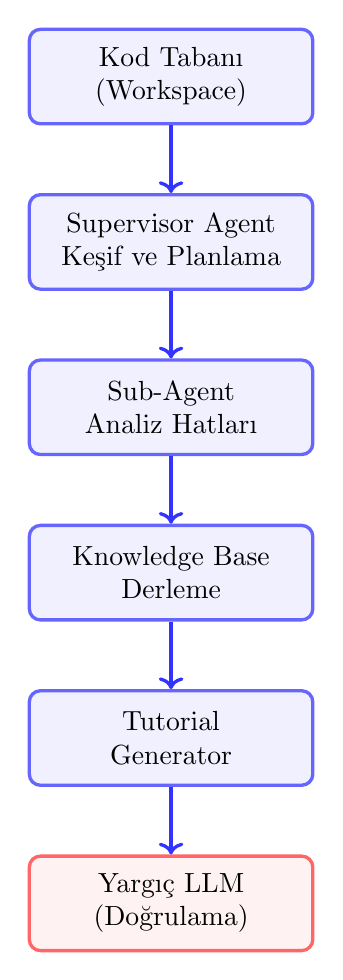
\begin{tikzpicture}[
        box/.style={rounded corners, draw=blue!60, fill=blue!6, very thick, minimum width=36mm, minimum height=12mm, align=center},
        flow/.style={->, very thick, draw=blue!80}
    ]
        \node[box] (input) at (0,0) {Kod Tabanı\\(Workspace)};
        \node[box] (analysis) at (0,-2.1) {Supervisor Agent\\Keşif ve Planlama};
        \node[box] (subpipe) at (0,-4.2) {Sub-Agent\\Analiz Hatları};
        \node[box] (kb) at (0,-6.3) {Knowledge Base\\Derleme};
        \node[box] (tutorial) at (0,-8.4) {Tutorial\\Generator};
        \node[box, fill=red!5, draw=red!60] (judge) at (0,-10.5) {Yargıç LLM\\(Doğrulama)};

        \draw[flow] (input) -- (analysis);
        \draw[flow] (analysis) -- (subpipe);
        \draw[flow] (subpipe) -- (kb);
        \draw[flow] (kb) -- (tutorial);
        \draw[flow] (tutorial) -- (judge);
    \end{tikzpicture}
    \caption{Bilgi üretim hattının üst düzey görünümü.}
    \label{fig:pipeline-overview}
\end{figure}

Mimari, iki aşamalı Sub-Agent kurgusu üzerine kuruludur. Supervisor Agent keşif, planlama ve orkestrasyon görevlerini yürütür; bağlam yükünü azaltmak için işleri Sub-Agent'lara devreder. Sub-Agent'lar kendi çalışma alanlarında ayrık olarak analiz yapar, bulgularını kalıcı depolara kaydeder ve Supervisor Agent’a raporlar. Supervisor Agent bu çıktıları birleştirerek nihai Knowledge Base'i oluşturur; ardından içerik üretimi için Tutorial Generator bileşenini tetikler.

Deterministik görev bölme yaklaşımıyla kaynak dosya altındaki ilk seviye klasörler ayrı Sub-Agent'lara atanır. Alternatif olarak Supervisor Agent, planlama parametreleri ve bir yapılacaklar listesi üzerinden görevleri dinamik biçimde güncelleyebilir. Sub-Agent'ların kod tabanına yalnızca okuma, kendi çalışma alanlarına ise yazma yetkisi vardır; böylece bağlam yönetimi ve çıktı doğrulaması sadeleşir.

\begin{figure}[htbp]
    \centering
    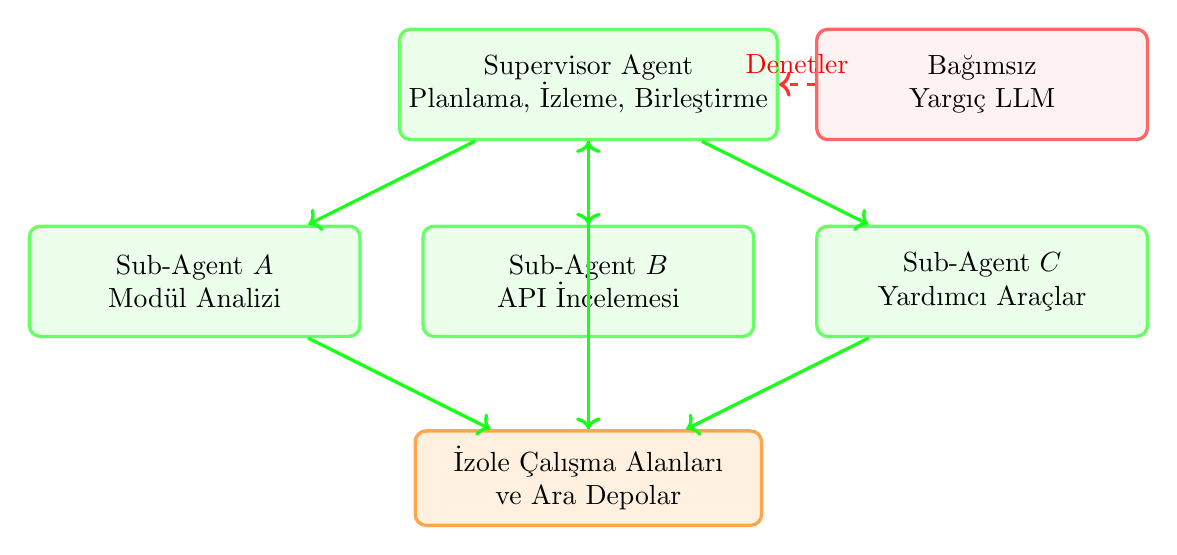
\begin{tikzpicture}[
        layer/.style={rounded corners, draw=green!60, fill=green!8, very thick, minimum width=42mm, minimum height=14mm, align=center},
        datastore/.style={rounded corners, draw=orange!70, fill=orange!12, very thick, minimum width=44mm, minimum height=12mm, align=center},
        flow/.style={->, very thick, draw=green!90}
    ]
        \node[layer] (main) at (7,4) {Supervisor Agent\\Planlama, İzleme, Birleştirme};
        \node[layer] (sub1) at (2,1.5) {Sub-Agent $A$\\Modül Analizi};
        \node[layer] (sub2) at (7,1.5) {Sub-Agent $B$\\API İncelemesi};
        \node[layer] (sub3) at (12,1.5) {Sub-Agent $C$\\Yardımcı Araçlar};
        \node[datastore] (stores) at (7,-1) {İzole Çalışma Alanları\\ve Ara Depolar};
        \node[layer, fill=red!5, draw=red!60] (judge) at (12, 4) {Bağımsız\\Yargıç LLM};

        \draw[flow] (main) -- (sub1);
        \draw[flow] (main) -- (sub2);
        \draw[flow] (main) -- (sub3);
        \draw[flow] (sub1) -- (stores);
        \draw[flow] (sub2) -- (stores);
        \draw[flow] (sub3) -- (stores);
        \draw[flow] (stores) -- (main);
        \draw[flow, dashed, draw=red!80] (judge) -- node[above, text=red]{Denetler} (main);
    \end{tikzpicture}
    \label{fig:agent-architecture}
\end{figure}


\noindent\textbf{Başarı Kriterleri ve Metrikler.}
Sistemin başarısı, teorik formüller yerine, sistem bileşenleri tarafından toplanan operasyonel veriler ve Yargıç LLM tarafından gerçekleştirilen kalite ölçümleri ile değerlendirilir.

\begin{itemize}
    \item \textbf{Operasyonel Verimlilik (Efficiency):} Sistemin bir projeyi analiz etme maliyeti şu üç temel metrikle izlenir:
    \begin{itemize}
        \item \textit{Token Tüketimi:} Toplam Girdi/Çıktı token sayısı (Maliyet analizi için).
        \item \textit{Süre (Duration):} Knowledge Base ve Tutorial fazlarının tamamlanma süreleri.
        \item \textit{Araç Kullanımı (Tool Calls):} Ajanların dosya okuma ve yazma sıklığı.
    \end{itemize}

    \item \textbf{İçerik Kalitesi (Yargıç LLM):} Üretilen eğitim içeriklerinin kalitesi, bağımsız bir LLM (Yargıç) tarafından 1-5 ölçeğinde puanlanır. Temel kriterler şunlardır:
    \begin{itemize}
        \item \textit{Doğruluk (Accuracy):} Kod örneklerinin gerçek kaynak kodla uyumu.
        \item \textit{Tamamlayıcılık (Completeness):} Konunun ne kadar kapsandığı.
        \item \textit{Pedagoji:} Anlatım sırasının mantıksal akışı.
    \end{itemize}

    \item \textbf{Süreç Dayanıklılığı (Robustness):}
    \begin{itemize}
        \item \textit{Bağlam Taşması (Context Overflow):} LLM'in hafıza sınırını aşma olaylarının sayısı.
        \item \textit{Toparlanma Başarısı:} Hata sonrası `retry` mekanizmasının başarı oranı.
    \end{itemize}
\end{itemize}


\section{Gereksinim Analizi}
\label{sec:gereksinim-analizi}

Gereksinimler üç düzeyde sınıflandırılmıştır: kullanıcı rolleri, sistem modülleri ve işlevsel akış. Sistemin iki temel kullanıcısı bulunmaktadır. Birincisi, Bilgi Bankası ve eğitim çıktıları üzerinden kod tabanını öğrenen geliştiricidir. İkincisi ise ajan süreçlerini başlatan, izleyen ve üretilen çıktının bütünlüğünü doğrulayan sistem operatörüdür. 

Sistem modülleri dört ana bileşenden oluşur. Supervisor Agent; keşif, planlama, görev dağıtımı ve Sub-Agent'lardan gelen çıktıları birleştirme görevlerini üstlenen merkezî unsurdur. Sub-Agent'lar; deterministik olarak veya koşula bağlı şekilde üretilen, belirli dizinleri veya görev kümelerini analiz eden ve izole çalışma alanlarında faaliyet gösteren ajanlardır. Knowledge Base deposu, tüm Sub-Agent özetlerinin toplandığı yapısal bir klasör düzeni sunarken, Tutorial Generator bileşeni bu Knowledge Base’i kullanarak pedagojik değer taşıyan eğitim materyallerini bağımsız bir çıktı klasörü altında üretir.

Sistemin işlevsel akışı ardışık beş aşamada gerçekleşir. İlk aşamada Supervisor Agent kod tabanının dosya yapısını çıkarır, kritik bileşenleri analiz eder ve deterministik ya da dinamik olarak görev listesini oluşturur. İkinci aşamada bu görevler ilgili Sub-Agent'lara dağıtılır. Üçüncü aşamada Sub-Agent'lar, sorumlu oldukları kod parçalarını inceleyerek özetlerini kendi çalışma dizinlerine kaydeder. Dördüncü aşamada Supervisor Agent bu alt çıktıları bir araya getirerek bütünleşik Knowledge Base’i oluşturur ve kalite kontrolünü gerçekleştirir. Son aşamada Tutorial Generator, oluşturulan bu Knowledge Base’i geliştiricilerin kolay öğrenebileceği bir pedagojik formata dönüştürür.

İşlevsel olmayan gereksinimler ise sistemin güvenlik, izlenebilirlik, genişletilebilirlik ve performans özelliklerini belirlemektedir. Sistem, özellikle dizin gezintisi (path traversal) zafiyetlerine karşı güvenli olacak şekilde tasarlanmalı; tüm API anahtarları gizli tutulmalı ve kod tabanına gömülmemelidir. Ayrıca ajanların karar verme süreçleri, özellikle görev delegasyonu  ve dosya işlemleri Phoenix aracı üzerinden ayrıntılı biçimde loglanmalıdır. Mimari, yeni araçların veya ajan türlerinin eklenmesine açık bir genişletilebilirlik sunmalıdır. Son olarak performans açısından, bir prototip olması nedeniyle süreç karmaşıklığını azaltmak amacıyla Sub-Agent'ların paralel değil, sıralı olarak çalıştırılması tercih edilmiştir.

\section{Fizibilite}
\label{sec:fizibilite}

\subsection{Teknik Fizibilite}
\label{sec:teknik-fizibilite}

\subsubsection{Donanım}
\label{sec:donanim-fizibilitesi}
Model eğitimi hedeflenmediği için yüksek donanım yatırımı gerekmez. LLM çağrıları API tabanlıdır; standart bir geliştirici bilgisayarı yeterlidir. İş yükü Sub-Agent'lara bölündüğü için bellek baskısı artmaz, uzun dosya okumaları engellenir.

\subsubsection{Yazılım}
\label{sec:yazilim-fizibilitesi}
\begin{itemize}
    \item \textbf{İşletim Sistemi:} Windows, macOS veya Linux.
    \item \textbf{Programlama Dili:} Python 3.10+ (Backend), TypeScript/React (Frontend).
    \item \textbf{Çerçeveler ve Araçlar:} \texttt{smolagents} (Ajan Orkestrasyonu), \texttt{LiteLLM} (AI Gateway), \texttt{Next.js} (Web Arayüzü), \texttt{Phoenix} (İzleme).
\end{itemize}

\subsection{Yasal Fizibilite}
\label{sec:yasal-fizibilite}
Kullanılan kütüphaneler MIT veya Apache~2.0 benzeri açık kaynak lisanslarıyla dağıtılır. Analiz edilecek kod tabanının proje ekibine ait olması veya lisans uyumunun sağlanması yeterlidir.

\subsection{Ekonomik Fizibilite}
\label{sec:ekonomik-fizibilitesi}

Projenin ekonomik fizibilitesi, düşük başlangıç maliyeti ve yüksek katma değer üretme potansiyeli sayesinde olumlu olarak değerlendirilmektedir. Sistem, büyük ölçüde açık kaynaklı yazılımlar ve bulut tabanlı LLM servisleri üzerine kurulu olup, merkezi ve sürekli bir altyapı yatırımı gerektirmemektedir.

\subsubsection{Giderler}

Temel bileşenler ücretsizdir. Maliyet kalemleri ağırlıklı olarak mühendislik eforu ve LLM API çağrılarından oluşmaktadır. Geliştirme ve test aşamalarında Google AI Studio veya OpenRouter üzerinden sunulan ücretsiz ya da düşük maliyetli modeller kullanılabilmektedir. Son kullanıcıya sunulan nihai dokümantasyon ve eğitim içeriklerinin üretiminde ise daha güçlü modeller tercih edilerek kalite–maliyet dengesi sağlanmaktadır.

Başlıca gider kalemleri aşağıda özetlenmiştir:

\begin{itemize}
    \item \textbf{Geliştirme Maliyeti:} Sistem mimarisi, çoklu ajan orkestrasyonu ve prompt mühendisliği için harcanan mühendislik eforu.
    \item \textbf{LLM API Maliyetleri:}
    \begin{itemize}
        \item \textit{Gemini 2.5 Pro:} Ortalama bir proje analizi için yaklaşık \$0.10 – \$0.50.
        \item \textit{GPT-OSS-120B:} Yüksek kalite gerektiren son tutorial üretimi aşamalarında sınırlı ve seçici kullanım.
    \end{itemize}
\end{itemize}

\subsubsection{Katma Değer}

Sistemin sağladığı katma değer, doğrudan parasal kazançtan ziyade zaman tasarrufu ve verimlilik artışı üzerinden ortaya çıkmaktadır. Bu bağlamda öne çıkan kazanımlar şunlardır:

\begin{itemize}
    \item Dokümantasyon ve proje öğrenme süreçlerinde \%80’den fazla zaman tasarrufu.
    \item Yeni geliştiricilerin projeye adaptasyon süresinin önemli ölçüde kısalması (hızlı onboarding).
    \item Kod tabanı değiştikçe ajanların yeniden çalıştırılmasıyla sürekli güncel dokümantasyon elde edilmesi.
    \item İlk kullanımda elde edilen zaman kazancı sayesinde sistemin kendi maliyetini kısa sürede amorti edebilmesi.
\end{itemize}

Bu yönleriyle proje, hem bireysel geliştiriciler hem de kurumsal yazılım ekipleri için ekonomik açıdan sürdürülebilir ve ölçeklenebilir bir çözüm sunmaktadır.

\subsection{İşgücü ve Zaman Fizibilitesi}
\label{sec:isgucu-zaman-fizibilitesi}

\textbf{Ekip:} 2 kişi (yazılım/araştırma odaklı).

\textbf{Genel Yaklaşım:} İlk sürüm için 8–12 hafta aralığında bir geliştirme süresi öngörülür. Detaylı şema şekil 2.2'de sunulmuştur.

\begin{figure}[H]
\centering
\begin{ganttchart}[
    hgrid,
    vgrid,
    x unit=0.45cm,
    y unit chart=0.6cm,
    bar height=0.45,
    bar label font=\scriptsize,
    bar/.append style={fill=gray!30},
]{1}{12}          % ← Haftalar (1–12)
    
    \gantttitle{İşgücü Gantt Şeması (12 Hafta)}{12} \\

    % Geliştirici
    \ganttgroup{Geliştirici}{1}{12} \\
    \ganttbar{Repo + Dosya Katmanı}{1}{2} \\
    \ganttbar{Sub-Agent Temelleri}{3}{4} \\
    \ganttbar{Loglama + Retry}{9}{10} \\

    % Araştırmacı
    \ganttgroup{Araştırmacı}{1}{12} \\
    \ganttbar{Knowledge Base + Şablonlar}{5}{6} \\
    \ganttbar{Eğitim Pipeline Tasarımı}{7}{8} \\

    % Ortak Görevler
    \ganttgroup{Ortak Görevler}{1}{12} \\
    \ganttbar{Sub-Agent Tasarım Konsepti}{3}{4} \\
    \ganttbar{E2E Test + Raporlama}{11}{12} \\

\end{ganttchart}
\caption{İşgücü Fizibilitesi – Rol Bazlı Gantt Şeması}
\end{figure}


\chapter{SİSTEM TASARIMI}
\label{ch:sistem-tasarimi}

Bu bölümde, geliştirilen çok ajanlı yapay zekâ analiz platformunun sistem tasarımı detaylandırılmaktadır. Tasarım mimarisi; kullanıcı etkileşimi, veri yönetimi ve nesne yönelimli modelleme olmak üzere üç temel eksende kurgulanmıştır. Amaç, karmaşık yazılım projelerini otonom olarak analiz edebilen ve eğitsel içerik üretebilen modüler, güvenli ve ölçeklenebilir bir yapı sunmaktır.

%---------------------------------------------------------
\section{Arayüz Tasarımı}
\label{sec:arayuz-tasarimi}

Sistem, kullanım kolaylığı ve operasyonel esnekliği bir arada sunmak amacıyla ikili bir arayüz yapısı benimsemiştir: Operasyonel süreçler için **Komut Satırı Arayüzü (CLI)** ve analitik çıktılar için **Web Tabanlı Kontrol Paneli**.

\subsection{Komut Satırı Arayüzü (CLI)}
Analiz süreçlerinin başlatılması ve yönetilmesi, geliştiricilerin alışkın olduğu terminal ortamı üzerinden gerçekleştirilir. Kullanıcılar, tek bir komut ile hedef projeyi sisteme tanıtır ve analiz sürecini başlatır. Sistemin CLI katmanı, arka planda çalışan yapay zekâ ajanlarının durumunu, kaynak tüketimini ve ilerleme yüzdelerini anlık olarak terminal ekranına yansıtır. Bu yalın tasarım, sistemin CI/CD (Sürekli Entegrasyon/Dağıtım) boru hatlarına kolayca entegre edilmesine olanak tanır.

\subsection{Web Tabanlı Kontrol Paneli (Web Dashboard)}
Otonom analiz tamamlandıktan sonra üretilen Knowledge Base ve eğitim materyallerinin son kullanıcıya sunulması için modern web teknolojileri (Next.js ve React) kullanılarak geliştirilmiş bir arayüz mevcuttur. Bu panelin temel işlevleri şunlardır:

\begin{itemize}
    \item **Proje Kütüphanesi:** Analiz edilen farklı kod tabanlarının görsel kartlar halinde listelenmesi ve yönetilmesi.
    \item **Etkileşimli İçerik Görüntüleyici:** Ajanlar tarafından üretilen Markdown formatındaki ders içeriklerinin, kod renklendirme (syntax highlighting) ve dinamik diyagram destekli olarak okunabilir hale getirilmesi.
    \item **Akıllı Gezinme:** Oluşturulan müfredat içerikleri arasında hiyerarşik geçiş imkanı.
\end{itemize}

Şekil~\ref{fig:ui-flow}'te sistemin operasyonel ve analitik arayüzleri arasındaki veri akış diyagramı sunulmuştur.

\begin{figure}[H]
    \centering
    \resizebox{0.95\textwidth}{!}{%
    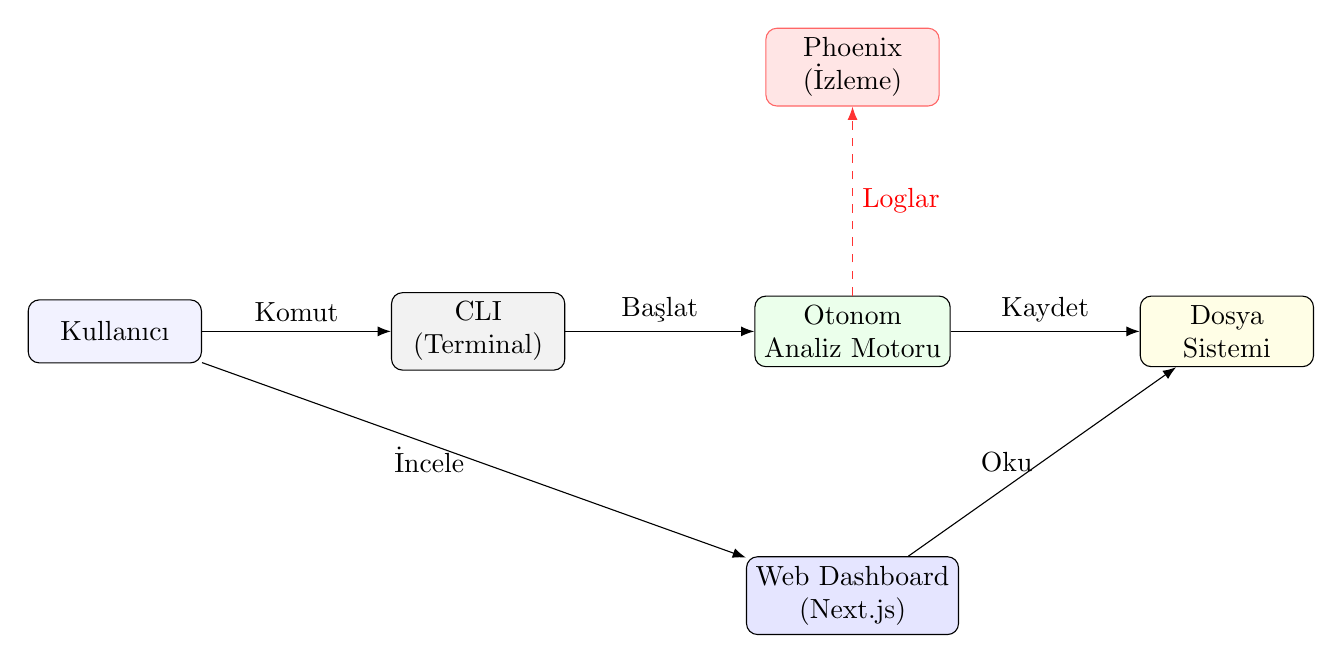
\begin{tikzpicture}[
        node distance=2.4cm,
        >=Latex,
        box/.style={
            draw,
            rounded corners,
            minimum width=22mm,
            minimum height=8mm,
            align=center,
            fill=blue!5
        }
    ]
        \node[box] (user) {Kullanıcı};
        \node[box, right=of user, fill=gray!10] (cli) {CLI\\(Terminal)};
        \node[box, right=of cli, fill=green!8] (pipeline) {Otonom\\Analiz Motoru};
        \node[box, above=of pipeline, fill=red!10, draw=red!60] (phoenix) {Phoenix\\(İzleme)};
        \node[box, right=of pipeline, fill=yellow!10] (fs) {Dosya\\Sistemi};
        \node[box, below=of pipeline, fill=blue!10] (web) {Web Dashboard\\(Next.js)};

        \draw[->] (user) -- node[above]{Komut} (cli);
        \draw[->] (cli) -- node[above]{Başlat} (pipeline);
        \draw[->] (pipeline) -- node[above]{Kaydet} (fs);
        \draw[->] (web) -- node[left]{Oku} (fs);
        \draw[->] (user) -- node[left]{İncele} (web);
        \draw[dashed, ->, draw=red!80] (pipeline) -- node[right, text=red]{Loglar} (phoenix);
    \end{tikzpicture}%
    }
    \caption{Kullanıcı etkileşimi ve veri akış şeması.}
    \label{fig:ui-flow}
\end{figure}

%---------------------------------------------------------
\section{Veri Yapısı Tasarımı}
\label{sec:veri-yapisi-tasarimi}

Proje mimarisinde, karmaşık veritabanı yönetim sistemleri yerine, taşınabilirlik ve şeffaflığı ön planda tutan, dosya sistemi tabanlı (filesystem-based) bir veri yaklaşımı tercih edilmiştir. Bu tasarım kararı, üretilen dokümantasyonun versiyon kontrol sistemleri (örn. Git) ile uyumlu olmasını ve projenin kendisiyle birlikte saklanabilmesini sağlar.

\subsection{Yapılandırma Yönetimi}
Sistemin davranış kalıpları ve parametreleri, merkezi yapılandırma dosyaları üzerinden yönetilir. Model seçimleri, API erişim anahtarları ve global sistem ayarları tek bir noktadan kontrol edilirken, web arayüzünde görüntülenecek metadata bilgileri ayrıştırılmış formatlarda saklanır.

\subsection{İzole Çalışma Alanları (Scoped Filesystem)}
Veri güvenliğini sağlamak ve projeler arası çakışmaları önlemek adına "İzole Dosya Sistemi" mimarisi uygulanmıştır. Her analiz süreci, kendine tahsis edilen üç katmanlı bir dizin yapısı içinde çalışır:

\begin{enumerate}
    \item **Kaynak Katmanı (Okuma):** Ajanların sadece okuma iznine sahip olduğu, orijinal kod tabanının bulunduğu güvenli alan.
    \item **Bellek Katmanı (Geçici):** Analiz sürecinde oluşturulan ara özetlerin ve notların tutulduğu çalışma alanı.
    \item **Çıktı Katmanı (Yazma):** Nihai eğitim materyallerinin ve raporların derlendiği sonuç klasörü.
\end{enumerate}

Bu yapı sayesinde, yapay zekâ ajanlarının proje dosyalarına zarar vermesi engellenmiş ve veri bütünlüğü garanti altına alınmıştır.

%---------------------------------------------------------
\section{Nesneye Yönelik Tasarım ve Ajan Mimarisi}
\label{sec:ajan-mimarisi}

Sistemin yazılım mimarisi, klasik statik sınıf hiyerarşileri yerine, esnekliği maksimize eden **Bileşimsel (Composition-based)** ve **Dinamik** bir tasarım modeline dayanır. Ajanlar, sabit kod blokları olarak değil, çalışma zamanında (runtime) ihtiyaca göre bir araya getirilen yetenek kümeleri olarak kurgulanmıştır.

\subsection{Dinamik Ajan Yapısı}
Platform içerisindeki her bir ajan (Supervisor Agent, Sub-Agent, Tutorial Generator), üç temel bileşenin dinamik birleşimiyle oluşturulur:

\begin{itemize}
    \item **Kimlik ve Rol Tanımı (Prompt):** Ajanın amacını, kurallarını ve davranış biçimini belirleyen doğal dil talimatlarıdır.
    \item **Yetenek Seti (Toolkit):** Ajanın dosya okuma, komut çalıştırma veya internette arama yapma gibi teknik becerilerini tanımlayan modüler fonksiyon kütüphaneleridir.
    \item **Dil Modeli (LLM):** Görevin karmaşıklığına göre seçilen, ajana zeka sağlayan işlem birimidir.
\end{itemize}

Bu modüler yapı, sisteme yeni yeteneklerin eklenmesini veya ajan davranışlarının değiştirilmesini, kaynak kodda köklü değişiklikler yapmadan mümkün kılar.

\subsection{Orkestrasyon Katmanı}
Ajanların koordinasyonu ve görev dağılımı, üst seviye yönetici sınıflar tarafından sağlanır. Sistemde ana yönetici rolünü üstlenen bu yapı, analiz sürecini mantıksal aşamalara (Bilgi Toplama, Planlama, İçerik Üretimi) böler ve her aşama için gerekli ajanları senkronize bir şekilde devreye sokar.

Şekil~\ref{fig:class-diagram}'de sistemin dinamik nesne mimarisi özetlenmiştir.

\begin{figure}[H]
    \centering
    \resizebox{0.85\textwidth}{!}{%
    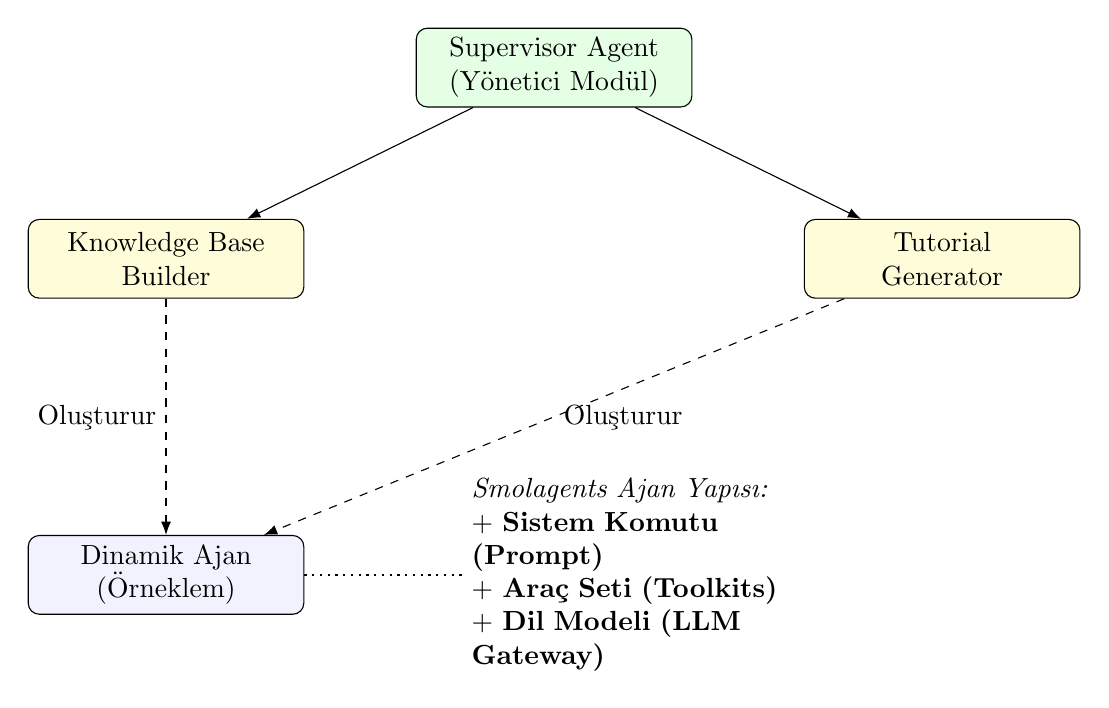
\begin{tikzpicture}[
        node distance=2.0cm,
        >=Latex,
        class/.style={
            draw,
            rounded corners,
            minimum width=35mm,
            minimum height=10mm,
            align=center,
            fill=blue!5
        }
    ]
        \node[class, fill=green!10] (orch) {Supervisor Agent\\(Yönetici Modül)};
        \node[class, below left=of orch, fill=yellow!15] (kb) {Knowledge Base\\Builder};
        \node[class, below right=of orch, fill=yellow!15] (tut) {Tutorial\\Generator};
        \node[class, below=of kb, yshift=-1cm] (agents) {Dinamik Ajan\\(Örneklem)};

        \draw[->] (orch) -- (kb);
        \draw[->] (orch) -- (tut);
        \draw[->, dashed] (kb) -- node[left]{Oluşturur} (agents);
        \draw[->, dashed] (tut) -- node[right]{Oluşturur} (agents);
        
        \node[right=of agents, text width=4.5cm, align=left] (components) {
            \textit{Smolagents Ajan Yapısı:}\\
            + \textbf{Sistem Komutu (Prompt)}\\
            + \textbf{Araç Seti (Toolkits)}\\
            + \textbf{Dil Modeli (LLM Gateway)}
        };
        \draw[dotted, thick] (agents) -- (components);
    \end{tikzpicture}%
    }
    \caption{Orkestrasyon yapısı ve dinamik ajan üretimi.}
    \label{fig:class-diagram}
\end{figure}

Bu mimari tercih, sistemin bakım maliyetini düşürmekte ve farklı programlama dilleri veya teknolojiler için kolayca özelleştirilebilmesine olanak tanımaktadır.
\chapter{UYGULAMA SONUÇLARI ve TESTLER}
\label{ch:uygulama-sonuclari}

\section{Uygulama Tanıtımı}
\label{sec:uygulama-tanitimi}

Geliştirilen sistem, son kullanıcıların karmaşık komut dizileriyle uğraşmadan, doğrudan doğal dil ve basit terminal konfigürasyonlarıyla çalıştırabileceği bir yapı sunmaktadır. Uygulama, ana dizinde bulunan çalıştırıcı betik üzerinden yönetilmektedir. Bu betik, gerekli ortam değişkenlerini yükler, sanal ortamı kontrol eder ve Python tabanlı komut satırı arayüzünü başlatır.

Kullanıcılar için iki temel çalışma modu tasarlanmıştır:
\begin{enumerate}
    \item \textbf{Deep Agent Modu:} Sub-Agent mimarisinin tam kapasiteyle çalıştığı, önce Knowledge Base oluşturup ardından eğitim içeriği üreten mod.
    \item \textbf{Baseline Modu:} Karşılaştırma amacıyla geliştirilen, Sub-Agent ve Knowledge Base kullanmadan doğrudan tek bir ajanın (ReAct mimarisi) tüm işi yapmaya çalıştığı mod.
\end{enumerate}

Sistem, otonom analiz ve içerik üretimi için yapılandırılmış komut setleri ile çalıştırılmaktadır. Kullanıcı, hedef kod tabanının yolunu belirterek analizi başlatabilir; karşılaştırma amaçlı olarak sistemin alt-ajan kullanmadan doğrudan tekil bir yapı üzerinden ilerlediği bir temel (baseline) modu da desteklenmektedir.

Uygulama çalıştığında, arka planda olay tabanlı bir loglama sistemi devreye girer. Kullanıcı terminalde anlık ilerlemeyi (ajanın o an hangi dosyayı okuduğu, hangi kararı verdiği) görebilirken, üretilen Markdown formatındaki eğitim dokümanları ve analiz raporları ilgili dizin altında otomatik olarak oluşturulur.

\section{Test Sonuçları}
\label{sec:test-sonuclari}

Sistemin başarımı, \textit{Sistem Analizi} bölümünde belirlenen gereksinimler doğrultusunda, özellikle maliyet etkinliği ve bağlam (context) yönetimi açısından test edilmiştir. Bu testlerde "Agent Lightning" kütüphanesi örnek proje olarak kullanılmış ve aynı donanım/ortam şartlarında hem Baseline hem de Deep Agent modları çalıştırılmıştır.

Elde edilen veriler, sistemin işlem yükü, token tüketimi ve araç kullanım sıklığı gibi performans metriklerini ortaya koymaktadır.

\subsection{Maliyet ve Bağlam Analizi (Deney 4)}

Büyük Dil Modelleri ile çalışan sistemlerde en kritik darboğaz, modelin bağlam penceresi ve token başına maliyettir. Aşağıdaki Tablo \ref{tab:cost-context}, Baseline ve Deep Agent yaklaşımlarının "Tutorial Üretim Fazı" için karşılaştırmalı performansını göstermektedir.

\begin{table}[htbp]
    \centering
    \caption{Baseline ve Deep Agent Modellerinin Tutorial Üretim Fazı Karşılaştırması}
    \label{tab:cost-context}
    \begin{tabular}{|l|c|c|}
        \hline
        \textbf{Metrik} & \textbf{Baseline Agent} & \textbf{Deep Agent} \\
        \hline
        Toplam Süre (saniye) & 378.25 & 620.98 \\
        \hline
        Girdi Token Sayısı (Input) & 1,732,968 & 3,236,280 \\
        \hline
        Çıktı Token Sayısı (Output) & 77,745 & 145,053 \\
        \hline
        Toplam Token Maliyeti & \textbf{1.81 Milyon} & \textbf{3.38 Milyon} \\
        \hline
        Araç Çağrı Sayısı (Tool Calls) & 32 & 43 \\
        \hline
        Bağlam Taşması (Overflow) & 0 & 0 \\
        \hline
    \end{tabular}
\end{table}

\noindent\textbf{Analiz:}
Tablo incelendiğinde, Deep Agent mimarisinin Baseline'a göre yaklaşık iki kat daha fazla token tükettiği ve işlemin daha uzun sürdüğü görülmektedir. İlk bakışta bu bir dezavantaj gibi görünse de, çıktının kalitesi ve derinliği göz önüne alındığında (Bkz. Bölüm \ref{sec:dogrulama}), bu "fazladan" maliyetin sisteme \textbf{bağlam zenginliği} olarak geri döndüğü anlaşılmaktadır. Baseline ajan, daha az token harcamasına rağmen yüzeysel ve genel geçer çıktılar üretirken; Deep Agent, oluşturduğu Knowledge Base'i bağlamına yüklediği için (input token artışı buradan kaynaklanmaktadır) çok daha detaylı, kod referanslı ve teknik doğruluğu yüksek içerikler üretmiştir.

Ayrıca, her iki sistemde de "Bağlam Taşması (Context Overflow)" olayının "0" olması, geliştirilen hız sınırlamalı dil modeli sarmalayıcısının ve token yönetim mekanizmasının başarılı bir şekilde çalıştığını kanıtlamaktadır.

\section{Doğrulama}
\label{sec:dogrulama}

Sistemin ürettiği çıktıların kalitesi ve kullanıcı gereksinimlerini karşılama düzeyi, güncel bir yöntem olan "Judge LLM" (Yargıç LLM) metodu ile doğrulanmıştır.

\subsection{Yargıç LLM Değerlendirmesi (Deney 2)}

Bu deneyde, SOTA (State-of-the-Art) kabul edilen \textbf{Claude 4.5 Sonnet} ve \textbf{GPT-OSS-120B} modelleri "tarafsız yargıç" olarak atanmıştır. Yargıçlara, hem Baseline (Seri A) hem de Deep Agent (Seri B) tarafından üretilen eğitim dokümanları, kaynak kod ile birlikte verilmiş ve şu üç kriterde puanlama yapmaları istenmiştir:

\begin{enumerate}
    \item \textbf{Doğruluk (Fidelity):} Üretilen kod örnekleri ve açıklamalar gerçek kod tabanıyla örtüşüyor mu? Halüsinasyon var mı?
    \item \textbf{Pedagoji (Pedagogy):} Anlatım, bir öğrencinin anlayabileceği şekilde basitten zora doğru mu? Örnekler öğretici mi?
    \item \textbf{Kapsam (Coverage):} Kod tabanının kritik özelliklerine değinilmiş mi yoksa sadece yüzeyde mi kalınmış?
\end{enumerate}

Yargıçların değerlendirme sonuçları Tablo \ref{tab:win-rate}’de özetlenmiştir.

\begin{table}[htbp]
    \centering
    \caption{Yargıç LLM'lerin Kalite Değerlendirmesi (5 üzerinden puan)}
    \label{tab:win-rate}
    \begin{tabular}{|l|c|c|c|c|c|c|}
        \hline
        \multirow{2}{*}{\textbf{Yargıç Model}} & \multicolumn{2}{c|}{\textbf{Doğruluk}} & \multicolumn{2}{c|}{\textbf{Pedagoji}} & \multicolumn{2}{c|}{\textbf{Kapsam}} \\
        \cline{2-7}
         & Base & \textbf{Deep} & Base & \textbf{Deep} & Base & \textbf{Deep} \\
        \hline
        Claude 4.5 Sonnet & 3 & \textbf{5} & 3 & \textbf{5} & 3 & \textbf{5} \\
        \hline
        GPT-OSS-120B & 4 & \textbf{5} & 4 & \textbf{5} & 4 & \textbf{5} \\
        \hline
    \end{tabular}
\end{table}

\begin{figure}[H]
    \centering
    \begin{tikzpicture}[scale=0.9]
        \begin{axis}[
            ybar,
            enlarge x limits=0.25,
            legend style={at={(0.5,-0.2)}, anchor=north, legend columns=-1},
            ylabel={Puan (1-5)},
            symbolic x coords={Doğruluk, Pedagoji, Kapsam},
            xtick=data,
            nodes near coords,
            nodes near coords align={vertical},
            ylimits={0,6},
            bar width=15pt,
            width=10cm,
            height=6cm,
            title={Ortalama Yargıç Değerlendirme Puanları}
        ]
            \addplot[fill=gray!40] coordinates {(Doğruluk,3.5) (Pedagoji,3.5) (Kapsam,3.5)};
            \addplot[fill=blue!40] coordinates {(Doğruluk,5.0) (Pedagoji,5.0) (Kapsam,5.0)};
            \legend{Baseline Agent, Deep Agent}
        \end{axis}
    \end{tikzpicture}
    \caption{Baseline ve Deep Agent modellerinin kalite metrikleri bazında karşılaştırılması.}
    \label{fig:evaluation-comparison}
\end{figure}

\noindent\textbf{Sonuç Yorumu:}
Her iki yargıç modeli de **Deep Agent (Seri B)** tarafından üretilen dokümanları "açık ara kazanan" (Winner: B) olarak ilan etmiştir.
\begin{itemize}
    \item \textbf{Doğruluk:} Baseline modelin, kullanılmayan (deprecated) API'leri önerdiği veya sınıf isimlerini yanlış yazdığı tespit edilmiştir. Deep Agent ise Knowledge Base'den doğrulama yaptığı için \%100'e yakın doğruluk sağlamıştır.
    \item \textbf{Pedagoji:} Deep Agent; "Hello World" örneğinden başlayıp, ileri seviye konulara (Distributed Training, Async Execution) doğru giden yapılandırılmış bir müfredat sunmuştur. Baseline ise konuları kopuk parçalar halinde sunmuştur.
\end{itemize}

\subsection{Gereksinim Uyumluluk Analizi}

Projenin başlangıcında (Bkz. Bölüm \ref{sec:gereksinim-analizi}) belirlenen işlevsel ve işlevsel olmayan gereksinimlerin karşılanma durumu yapılan son denetimlerle (audit) doğrulanmıştır.

\begin{itemize}
    \item \textbf{Sub-Agent Mimarisi:} \checkmark Tamamlandı. Supervisor Agent dinamik olarak Sub-Agent'lar oluşturabilmekte ve izole çalışma alanlarını yönetebilmektedir.
    \item \textbf{Güvenlik (Path Traversal):} \checkmark Tamamlandı. Geliştirilen kısıtlanmış dosya erişim modülü, ajanların sadece izin verilen dizinlere erişmesini garanti altına almıştır.
    \item \textbf{Knowledge Base Üretimi:} \checkmark Tamamlandı. Kod tabanından otomatik olarak kapsamlı bir Markdown Knowledge Base oluşturulabilmektedir.
    \item \textbf{Raporlama ve İzleme:} \checkmark Tamamlandı. Hem terminal çıktıları hem de JSON formatındaki metrik dosyaları ile süreç şeffaf hale getirilmiştir.
\end{itemize}

Bu sonuçlar, geliştirilen sistemin hedeflenen otonom eğitim içerik üretimi görevini başarıyla yerine getirdiğini ve Deep Agent mimarisinin, geleneksel yöntemlere göre kalite açısından belirgin bir üstünlük sağladığını doğrulamaktadır.

\chapter{SONUÇ VE TARTIŞMA}
\label{ch:sonuc-ve-tartisma}

Bu çalışmada, büyük ve karmaşık kod tabanlarını otomatize etmek amacıyla "Sub-Agent" mimarisine dayalı otonom bir yapay zekâ sistemi tasarlanmış ve prototipi geliştirilmiştir. Geliştirilen sistem, "Agent Lightning" gibi modern ve dokümantasyonu sınırlı kütüphaneler üzerinde test edilmiş; elde edilen sonuçlar hem nicel metrikler hem de nitel Yargıç LLM değerlendirmeleriyle analiz edilmiştir.

Proje kapsamında elde edilen temel sonuçlar ve tartışma başlıkları aşağıda sunulmuştur:

\section{Elde Edilen Kazanımlar}

\begin{enumerate}
    \item \textbf{Bağlam Sınırının Aşılması:} Geleneksel tek ajanlı sistemlerin en büyük problemi olan "bağlam penceresi" (context window) kısıtı, geliştirdiğimiz iki aşamalı (Knowledge Base Üretimi $\rightarrow$ İçerik Üretimi) mimari sayesinde aşılmıştır. Supervisor Agent'ın tüm dosyaları okumak yerine, görevi alt ajanlara dağıtması ve sadece özet bilgiyi (Knowledge Base) kullanması, sistemin binlerce dosyalık projelerde bile "bağlam taşması" yaşamadan çalışmasını sağlamıştır.

    \item \textbf{Kalite ve Derinlik Artışı:} Yapılan karşılaştırmalı testler (Bölüm \ref{sec:test-sonuclari}), Deep Agent stratejisinin token maliyetini artırmasına rağmen (Baseline: 1.8M vs Deep: 3.3M), çıktı kalitesinde tartışılmaz bir üstünlük sağladığını göstermiştir. Baseline ajan yüzeysel bilgiler verirken; Deep Agent, kodun derinliklerindeki mimari desenleri, asenkron çalışma yapılarını ve doğru sınıf isimlerini tespit ederek "kullanılabilir ve doğru" eğitim materyali üretmeyi başarmıştır. Yargıç LLM'ler, Deep Agent'a doğruluk ve pedagoji kriterlerinde tam puan (5/5) vermiştir.

    \item \textbf{Güvenli ve İzole Çalışma:} Tasarlanan kısıtlanmış dosya erişim modeli sayesinde, otonom ajanların sadece kendilerine atanan dizinlerde çalışması sağlanmış, böylece olası veri kaybı veya dizin gezintisi (path traversal) zafiyetleri mimari düzeyde engellenmiştir.
\end{enumerate}

\section{Kısıtlar ve Maliyet}

Sistemin sunduğu yüksek kalitenin bir bedeli olarak işlem süresi ve maliyeti artış göstermiştir. Deep Agent modunda bir kütüphanenin analizi ve tutorial üretimi ortalama 10-20 dakika sürmektedir. Bu süre, bir insanın haftalar süren öğrenme sürecine göre ihmal edilebilir olsa da, anlık yanıt bekleyen interaktif senaryolar için (örneğin IDE içi kod tamamlama) bu mimari şu an için yavaş kalabilir. Ayrıca token tüketiminin yüksek olması, GPT-OSS-120B gibi pahalı modellerle çalışıldığında maliyetli olabilir; bu nedenle sistemin Gemini 2.5 Pro veya açık kaynaklı (OSS) modellerle optimize edilmesi önerilmektedir.

\section{Gelecek Çalışmalar}

Mevcut prototipin başarısı, bu alanda yapılacak ileri çalışmalar için güçlü bir temel oluşturmaktadır. Gelecek dönemde şu geliştirmelerin yapılması hedeflenmektedir:

\begin{itemize}
    \item \textbf{İnsan Deneyleri:} Şu an Yargıç LLM'lerle yapılan doğrulamanın, gerçek yazılım geliştiriciler ve üniversite öğrencileriyle yapılacak A/B testleriyle (Deney 1 ve Deney 3) desteklenmesi.
    \item \textbf{Ablasyon Çalışmaları:} Bilgi Bankası bileşeninin etkisini daha net ölçmek için, sistemin farklı modüllerinin kapatılarak (ör. sadece RAG ile, Knowledge Base olmadan) test edilmesi (Deney 5).
    \item \textbf{Web Arayüzü:} Mevcut CLI yapısının, daha geniş kitlelere hitap edecek, sürükle-bırak özellikli bir Web UI ile zenginleştirilmesi.
\end{itemize}

Sonuç olarak, bu proje ile otonom ajanların sadece kod yazmakla kalmayıp, yazılan kodu "anlatma ve öğretme" konusunda da insan geliştiricilere güçlü bir asistan olabileceği kanıtlanmıştır.

\fi
\ifnum\projecttype=3
\input {LatexTutorial/kilavuz}
\fi

%%%%%%%%%%%%%%%%%%%%%%%%%%%%%%%%%%%%%%%%%%%%%%%%%%%%%
%%%%%%%%%%%%%%%      APPENDICES     %%%%%%%%%%%%%%%%%
%%%%%%%%%%%%%%%%%%%%%%%%%%%%%%%%%%%%%%%%%%%%%%%%%%%%%
\newpage\appendix
% gerekliyse ekler için aşağıdaki yorum satırlarını açabilirsiniz. 
%\input {projectChapters/A-appendix.tex}
%\input {projectChapters/B-appendix.tex}


%%%%%%%%%%%%%%%%%%%%%%%%%%%%%%%%%%%%%%%%%%%%%%%%%%%%%
%%%%%%%%%%%         BACK PAGES       %%%%%%%%%%%%%%%%
%%%%%%%%%%%%%%%%%%%%%%%%%%%%%%%%%%%%%%%%%%%%%%%%%%%%%
\newpage
\addcontentsline{toc}{chapter}{\bibName}
\singlespacing
\printbibliography[title={\bibName}]

\ifnum\final=1
\newpage
\addcontentsline{toc}{chapter}{\cvName}

\ifnum\projecttype>0
\input {cv.tex}
\fi
\fi

\end{document}